\documentclass[11pt,a4paper]{article}
\usepackage[margin=18mm,headheight=16pt]{geometry}
\usepackage[T1]{fontenc}
\usepackage{lmodern}
\usepackage{microtype}
\usepackage{graphicx}
\usepackage{booktabs}
\usepackage{tabularx}
\usepackage{longtable}
\usepackage{array}
\usepackage{enumitem}
\usepackage{xcolor}
\usepackage{amsmath}
\usepackage{amssymb}
\usepackage{titlesec}
\usepackage{hyperref}
\usepackage{caption}
\usepackage{float}
\usepackage{needspace}
\graphicspath{{../../images/}}

\definecolor{navy}{HTML}{12304A}
\definecolor{blue}{HTML}{147EA8}
\definecolor{ice}{HTML}{EAF6FA}
\definecolor{green}{HTML}{177A5B}
\definecolor{amber}{HTML}{A95E00}
\definecolor{red}{HTML}{A32121}
\definecolor{gray}{HTML}{5F6B73}
\definecolor{line}{HTML}{CDD8DE}

\hypersetup{colorlinks=true,linkcolor=navy,urlcolor=blue,pdftitle={Spacesuit Thermal Shielding Kit},pdfauthor={Timon Karl-Heinz Schwarz and SPHERE project team}}
\pagestyle{empty}
\titleformat{\section}{\Large\bfseries\color{navy}}{\thesection}{0.7em}{}
\titleformat{\subsection}{\large\bfseries\color{navy}}{\thesubsection}{0.7em}{}
\titlespacing*{\section}{0pt}{1.3em}{0.55em}
\titlespacing*{\subsection}{0pt}{1em}{0.35em}
\setlist[itemize]{leftmargin=1.4em,itemsep=0.25em,topsep=0.35em}
\setlist[enumerate]{leftmargin=1.7em,itemsep=0.35em,topsep=0.35em}
\captionsetup{font=small,labelfont=bf,labelsep=period}
\setlength{\parindent}{0pt}
\setlength{\parskip}{0.45em}
\renewcommand{\arraystretch}{1.18}
\newcolumntype{Y}{>{\raggedright\arraybackslash}X}
\newcolumntype{C}[1]{>{\centering\arraybackslash}p{#1}}

\newcommand{\safety}[1]{\par\noindent{\color{red}\textbf{SAFETY - }}#1\par}
\newcommand{\control}[1]{\par\noindent{\color{green}\textbf{CONTROL - }}#1\par}
\newcommand{\note}[1]{\par\noindent{\color{amber}\textbf{NOTE - }}#1\par}

\begin{document}

\begin{titlepage}
  \thispagestyle{empty}
  \begin{minipage}[t]{0.64\textwidth}
    {\color{blue}\large SPHERE}\par
    \vspace{8mm}
    {\fontsize{30}{34}\selectfont\bfseries\color{navy} Spacesuit Thermal Shielding Kit}\par
    \vspace{2mm}
    {\fontsize{20}{24}\selectfont\bfseries Standard Operating Procedure}\par
    \vspace{7mm}
    {\large Comparative Heat Transfer and Insulation Performance Laboratory}\par
    \vspace{8mm}
    \begin{tabular}{@{}ll@{}}
      \textbf{Document owner:} & Timon Karl-Heinz Schwarz \\
      \textbf{Project team:} & Piyath Vithanage, Elio Krollpfeiffer, \\
       & Dilan Fernando, Nuhansee Migelhewage \\
      \textbf{Issue date:} & 9 September 2026 \\
      \textbf{Planned duration:} & 30 minutes per group \\
    \end{tabular}
  \end{minipage}\hfill
  \begin{minipage}[t]{0.30\textwidth}
    \vspace{-4mm}
    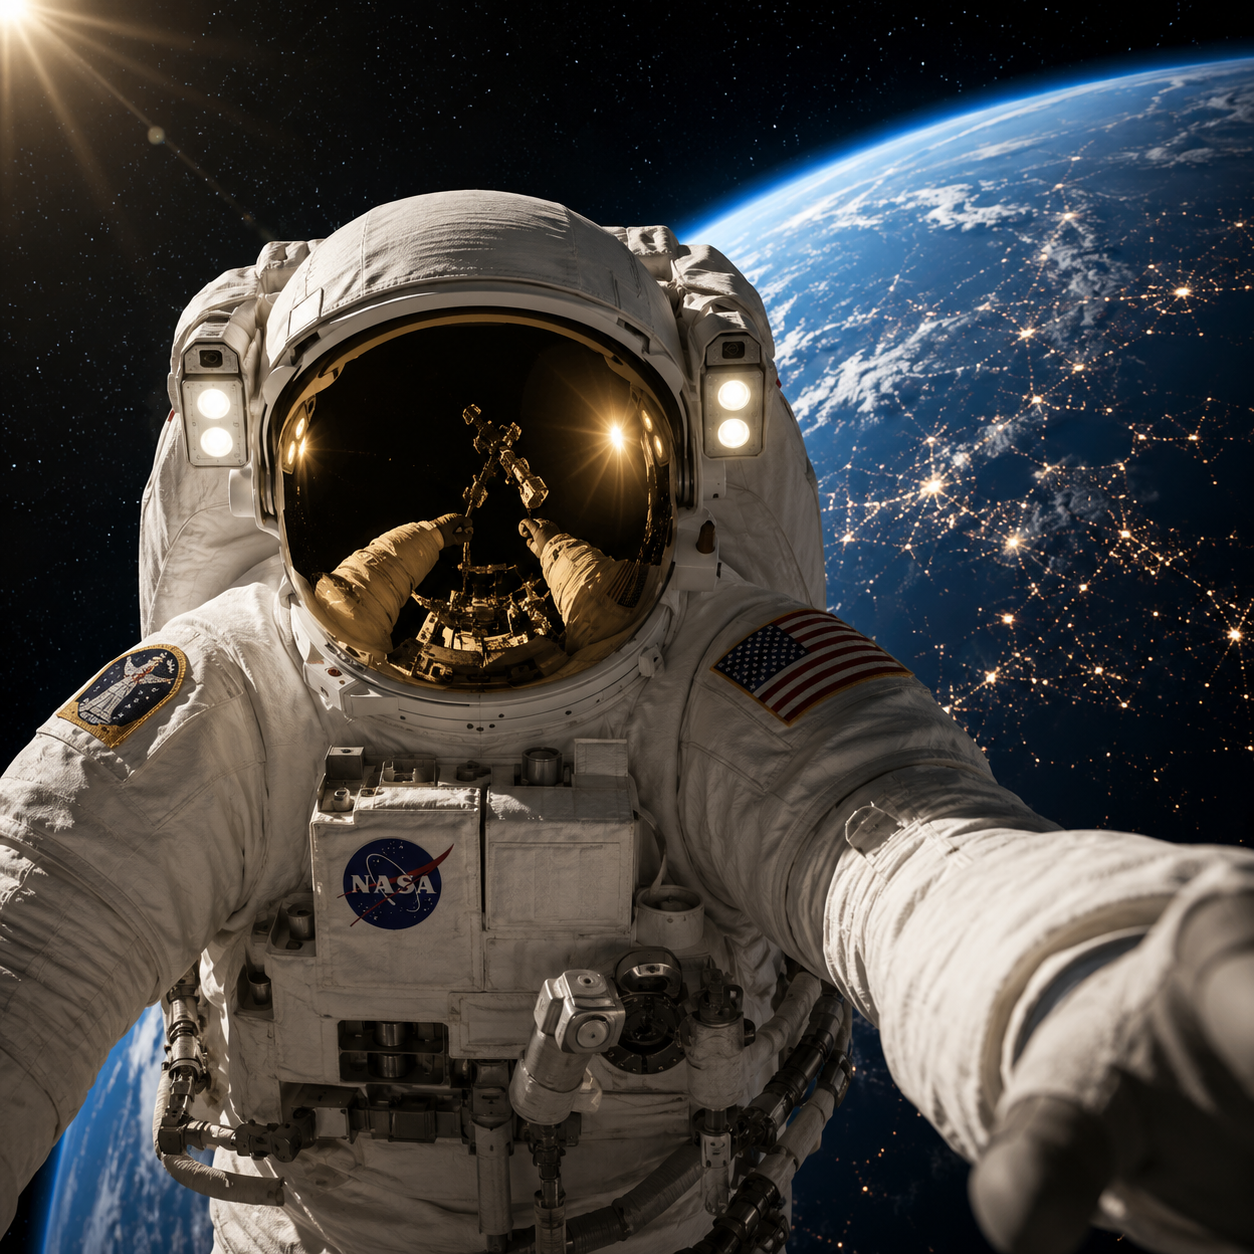
\includegraphics[width=\linewidth]{astronaut.png}
  \end{minipage}

  \vfill
  {\color{navy}\rule{\textwidth}{1.2pt}}\par
  \vspace{4mm}
  \textbf{Purpose.} This procedure enables four student teams to compare the transient cooling of identical, sealed 100 mL glass-jar capsules protected by bare, bubble-wrap, Mylar, and multilayer test configurations. It aligns the physical experiment with the current SPHERE student manual, teacher manual, task sheet, flashcards, and Mission Control model.

  \safety{Only the instructor or another designated adult may prepare and dispense hot water. The maximum initial water temperature is $80.0\,^{\circ}\mathrm{C}$. Never use boiling water. Eye protection and heat-resistant gloves are required.}
\end{titlepage}

\tableofcontents
\clearpage

\Needspace{8\baselineskip}
\section{Scope and learning outcomes}

This is an educational analog for comparing heat-transfer mechanisms and effective insulation performance. The glass jars, cotton, bubble wrap, and reflective film are not flight-qualified hardware, and an ice-water bath does not reproduce a space vacuum. The experiment instead provides a repeatable cold boundary for model comparison.

After the activity, students should be able to distinguish conduction, convection, and radiation; apply Newton's law of cooling; record a controlled temperature time series; calculate residuals and mean absolute error (MAE); and explain how leakage, probe placement, layer compression, and boundary drift affect repeatability.

\Needspace{8\baselineskip}
\section{Roles and stop-work authority}

\begin{tabularx}{\textwidth}{>{\bfseries}p{0.22\textwidth}Y}
\toprule
Role & Responsibility \\
\midrule
Instructor & Complete the local risk assessment; supervise hot-water handling; verify jar condition, probe-lid seals, ice-bath temperature, and safe separation of water from electronics. \\
Student teams & Assemble the assigned insulation configuration, record measurements exactly on schedule, report anomalies immediately, and keep the work area dry. \\
Timekeeper/data lead & Start the timer at immersion, announce 60-second intervals, enter values in Mission Control and the task sheet, and document any late or missed reading. \\
All participants & Stop the test immediately if a jar cracks or leaks, insulation becomes saturated, a probe moves, water reaches electronics, or any person is at risk. \\
\bottomrule
\end{tabularx}

\Needspace{8\baselineskip}
\section{Equipment and materials}

\begin{figure}[H]
\centering
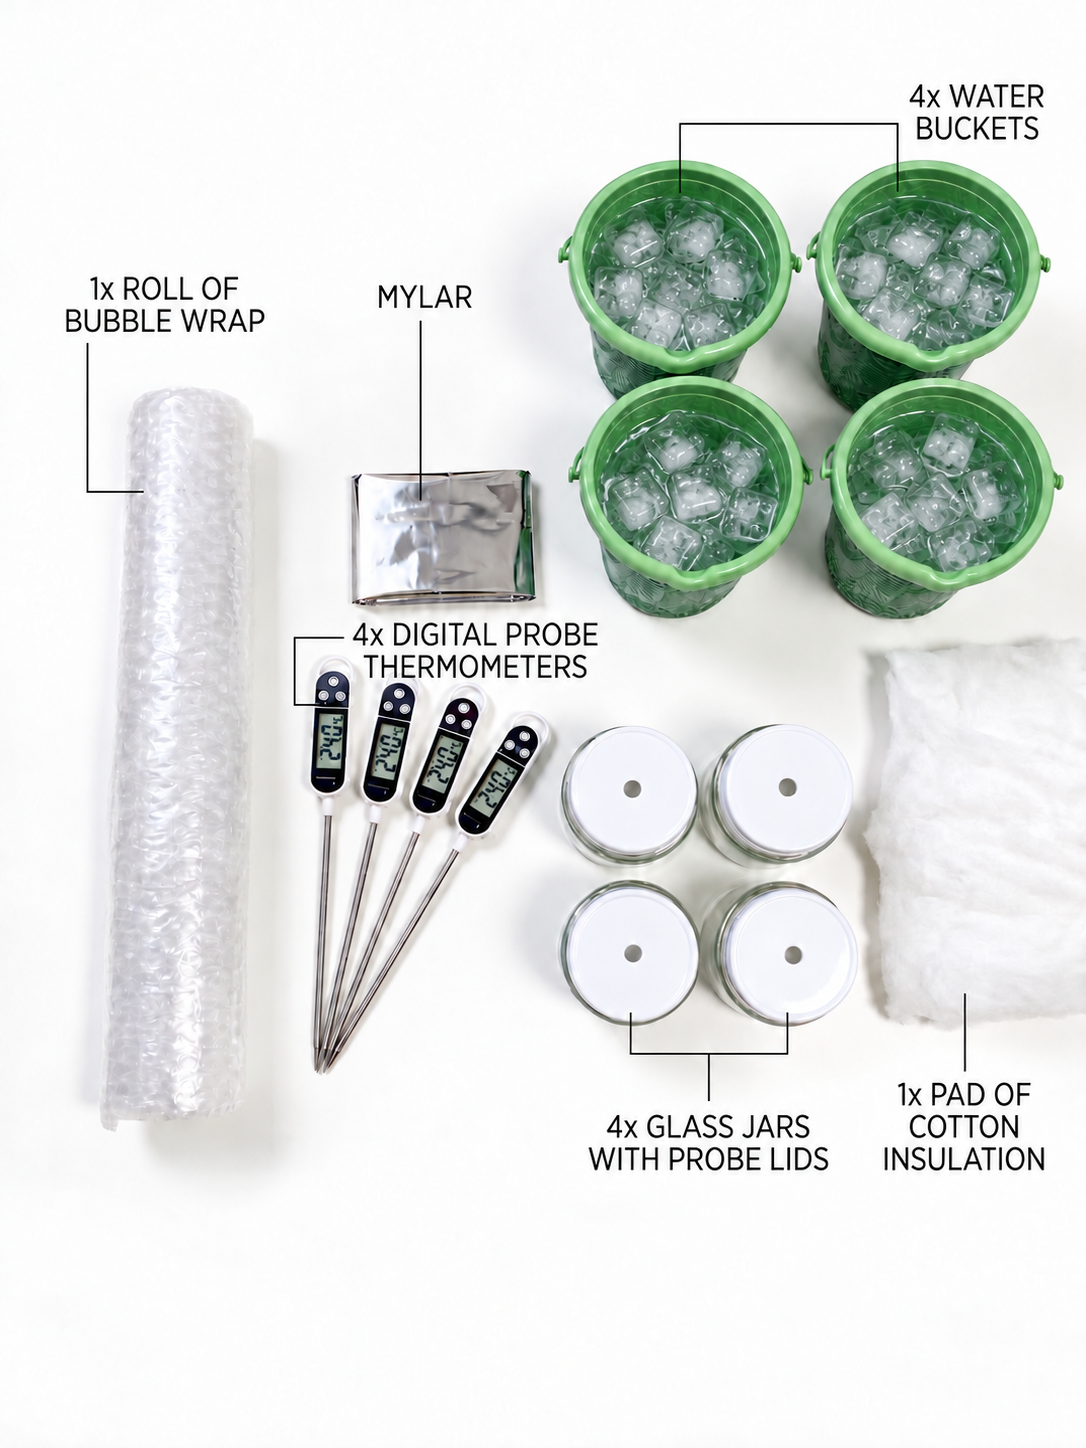
\includegraphics[height=0.50\textheight]{equipments.png}
\caption{Current SPHERE toolkit: four glass jars with prepared probe lids, four probe thermometers, four ice-water containers, cotton, bubble wrap, and Mylar.}
\end{figure}

\begin{longtable}{C{12mm}p{0.34\textwidth}p{0.50\textwidth}}
\toprule
\textbf{Qty.} & \textbf{Item} & \textbf{Requirement} \\
\midrule
\endhead
4 & 100 mL wide-mouth glass jars with prepared probe lids & Heat-safe, undamaged, identical geometry. The lid opening must support the probe and the approved classroom sealing method. \\
4 & Waterproof digital probe thermometers & Stainless-steel probe; nominal accuracy documented by the instructor (the manuals use $\pm0.5\,^{\circ}\mathrm{C}$ as the reference). \\
4 & Ice-water bath containers & Stable and deep enough for the external water line to remain above the internal capsule water level. \\
1 set & Cotton, bubble wrap, reflective Mylar, tape or elastic bands & Dry, reusable where practical, and applied consistently without crushing trapped-air layers. \\
1 & Supervised hot-water source and measuring vessel & Instructor use only; prepare no hotter than $80.0\,^{\circ}\mathrm{C}$. \\
1+ & Bath thermometer & Independent measurement of the actual environmental boundary temperature $T_{\mathrm{env}}$. \\
-- & Eye protection, heat-resistant gloves, towels, timer, worksheets & Required before the hot-water phase begins. Keep computers and electrical connections at a separate dry station. \\
\bottomrule
\end{longtable}

\begin{figure}[H]
\centering
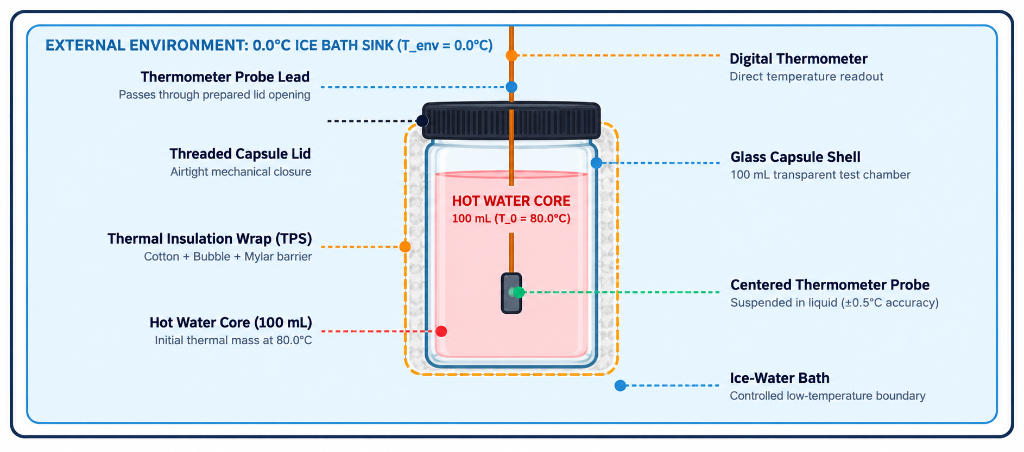
\includegraphics[width=0.96\textwidth]{hardware-schematic.png}
\caption{Glass-jar capsule arrangement and centered probe placement. The probe tip must remain clear of the lid, wall, and base.}
\end{figure}

\Needspace{8\baselineskip}
\section{Safety controls}

\safety{Hot water can cause scalding. Do not exceed $80.0\,^{\circ}\mathrm{C}$, do not use boiling water, and do not allow students to pour hot water unless the local risk assessment explicitly permits it under direct supervision.}

\begin{itemize}
  \item Inspect every glass jar and lid before use. Reject chipped, cracked, scratched, or poorly fitting components.
  \item Perform the seal check with cold water before introducing hot water. Use only the approved classroom lid-sealing method; do not improvise a pressure seal.
  \item The capsule is closed to resist leakage but is not a pressure vessel. Do not overfill, pressurize, or aim it toward a person.
  \item Wear eye protection. Use heat-resistant gloves or suitable tongs for filling, closing, transferring, immersing, and removing a warm capsule.
  \item Keep the bath below waist height on a stable surface. Wipe spills immediately and keep cables, displays, computers, and power supplies dry.
  \item Only the intended waterproof metal probe may contact water. The display, connector, and lead junction remain dry.
  \item If room conditions make $80\,^{\circ}\mathrm{C}$ unsuitable, use $55$--$60\,^{\circ}\mathrm{C}$ or room-temperature bath testing and enter the actual $T_0$ and $T_{\mathrm{env}}$ in Mission Control.
\end{itemize}

\Needspace{8\baselineskip}
\section{Pre-flight preparation}

\begin{figure}[H]
\centering
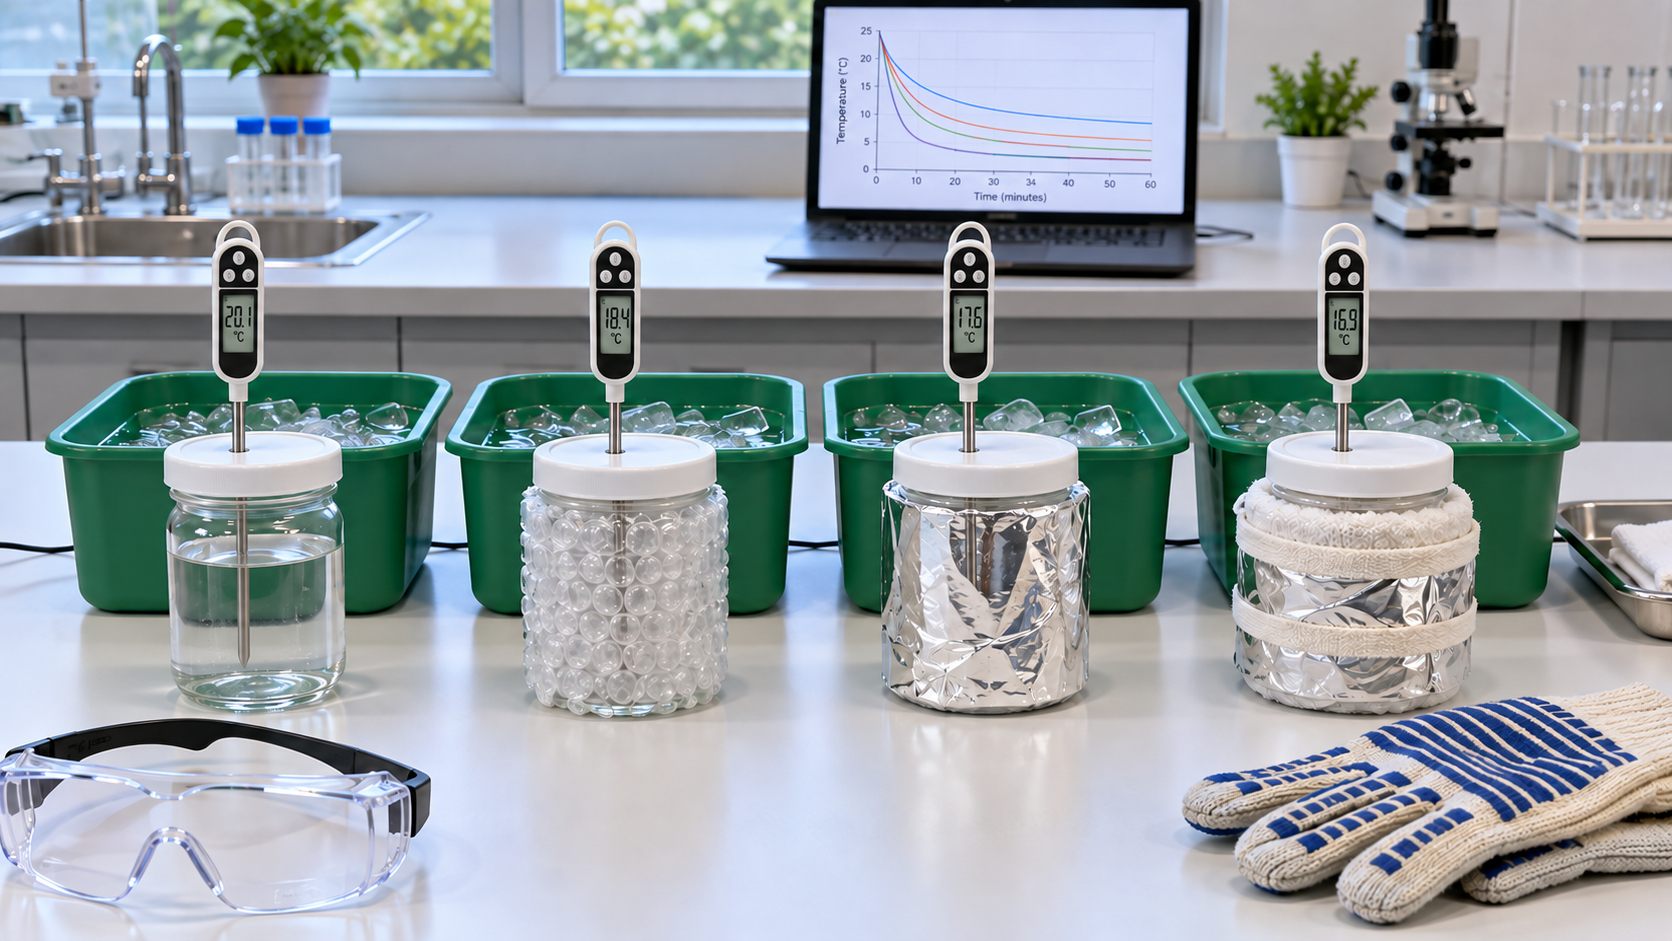
\includegraphics[width=0.96\textwidth]{preflight-thermal-lab.png}
\caption{Project-specific pre-flight arrangement showing the four glass-jar insulation configurations, ice-water baths, matching probe thermometers, PPE, and a separate dry data station.}
\end{figure}

\begin{enumerate}
  \item Confirm that the risk assessment, PPE, dry electronics station, towels, and emergency response arrangements are in place.
  \item Fill each jar with cold water, fit the probe through its prepared lid, secure the opening using the approved classroom method, close the lid, and invert briefly over a sink or secondary container. Reject or reseal any leaking capsule.
  \item Set the probe tip at the vertical center of the 100 mL water volume. Mark or clamp the lead so the depth cannot change.
  \item Prepare a well-mixed ice-water slurry. Measure and record the actual bath temperature; do not assume it is exactly $0.0\,^{\circ}\mathrm{C}$.
  \item Assign configurations A--D. Use identical water mass, jar geometry, probe depth, bath depth, timing, and handling.
\end{enumerate}

\control{A fair comparison requires the same measured starting temperature tolerance, water volume, probe position, immersion depth, bath condition, and 60-second observation interval for every configuration.}

\Needspace{15\baselineskip}
\section{Insulation configurations}

The constants below are educational reference-model values, not certified material properties and not guaranteed experimental results. The symbol $k$ is an effective system cooling constant; it is not thermal conductivity.

\begin{tabularx}{\textwidth}{p{0.19\textwidth}C{22mm}Yp{0.25\textwidth}}
\toprule
\textbf{Configuration} & \textbf{$k$ (min$^{-1}$)} & \textbf{Construction} & \textbf{Model $T(15)$} \\
\midrule
A Bare control & 0.150 & Uninsulated glass jar. & $8.4\,^{\circ}\mathrm{C}$ \\
B Bubble wrap & 0.040 & Two even layers with intact cells; close around the lid without compressing the air pockets. & $43.9\,^{\circ}\mathrm{C}$ \\
C Mylar & 0.121 & One complete reflective layer, shiny side outward. Avoid tears and direct water paths. & $13.0\,^{\circ}\mathrm{C}$ \\
D Multilayer assembly & 0.015 & Inner cotton spacer, middle bubble wrap, outer reflective Mylar; secure each layer independently. & $63.9\,^{\circ}\mathrm{C}$ \\
\bottomrule
\end{tabularx}

The listed temperatures use $T_0=80.0\,^{\circ}\mathrm{C}$ and $T_{\mathrm{env}}=0.0\,^{\circ}\mathrm{C}$. Cotton-only may be added as an optional fifth trial, but it is not one of the four standard comparison cases.

\begin{figure}[H]
\centering
\begin{minipage}[t]{0.235\textwidth}\centering
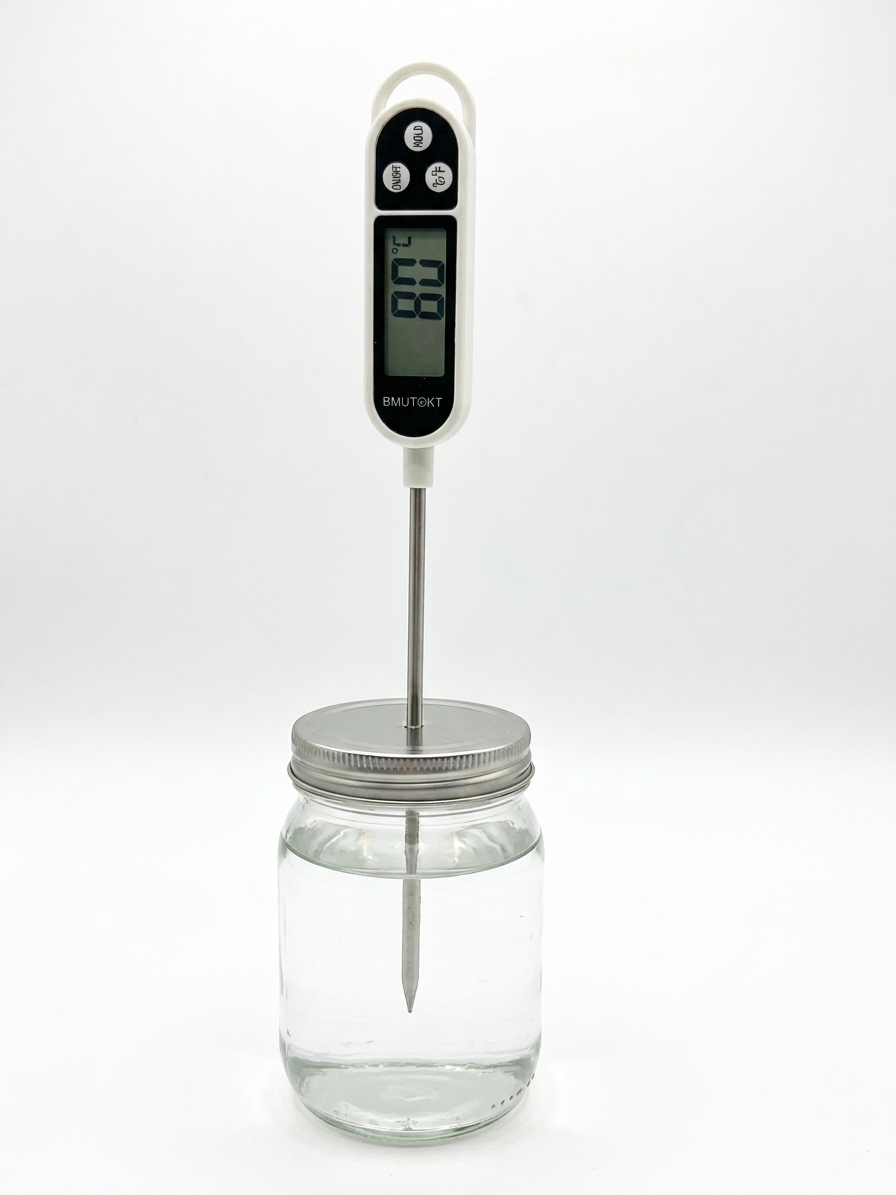
\includegraphics[height=42mm]{barecapsule.jpeg}\\[-1mm]\small A. Bare glass capsule
\end{minipage}\hfill
\begin{minipage}[t]{0.235\textwidth}\centering
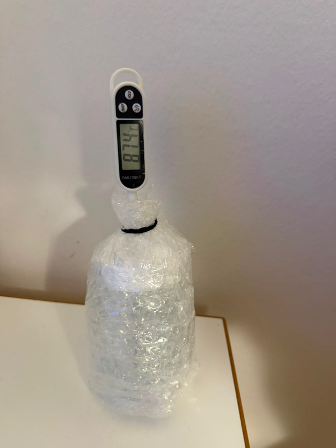
\includegraphics[height=42mm]{bubblewrap-only.png}\\[-1mm]\small B. Bubble wrap
\end{minipage}\hfill
\begin{minipage}[t]{0.235\textwidth}\centering
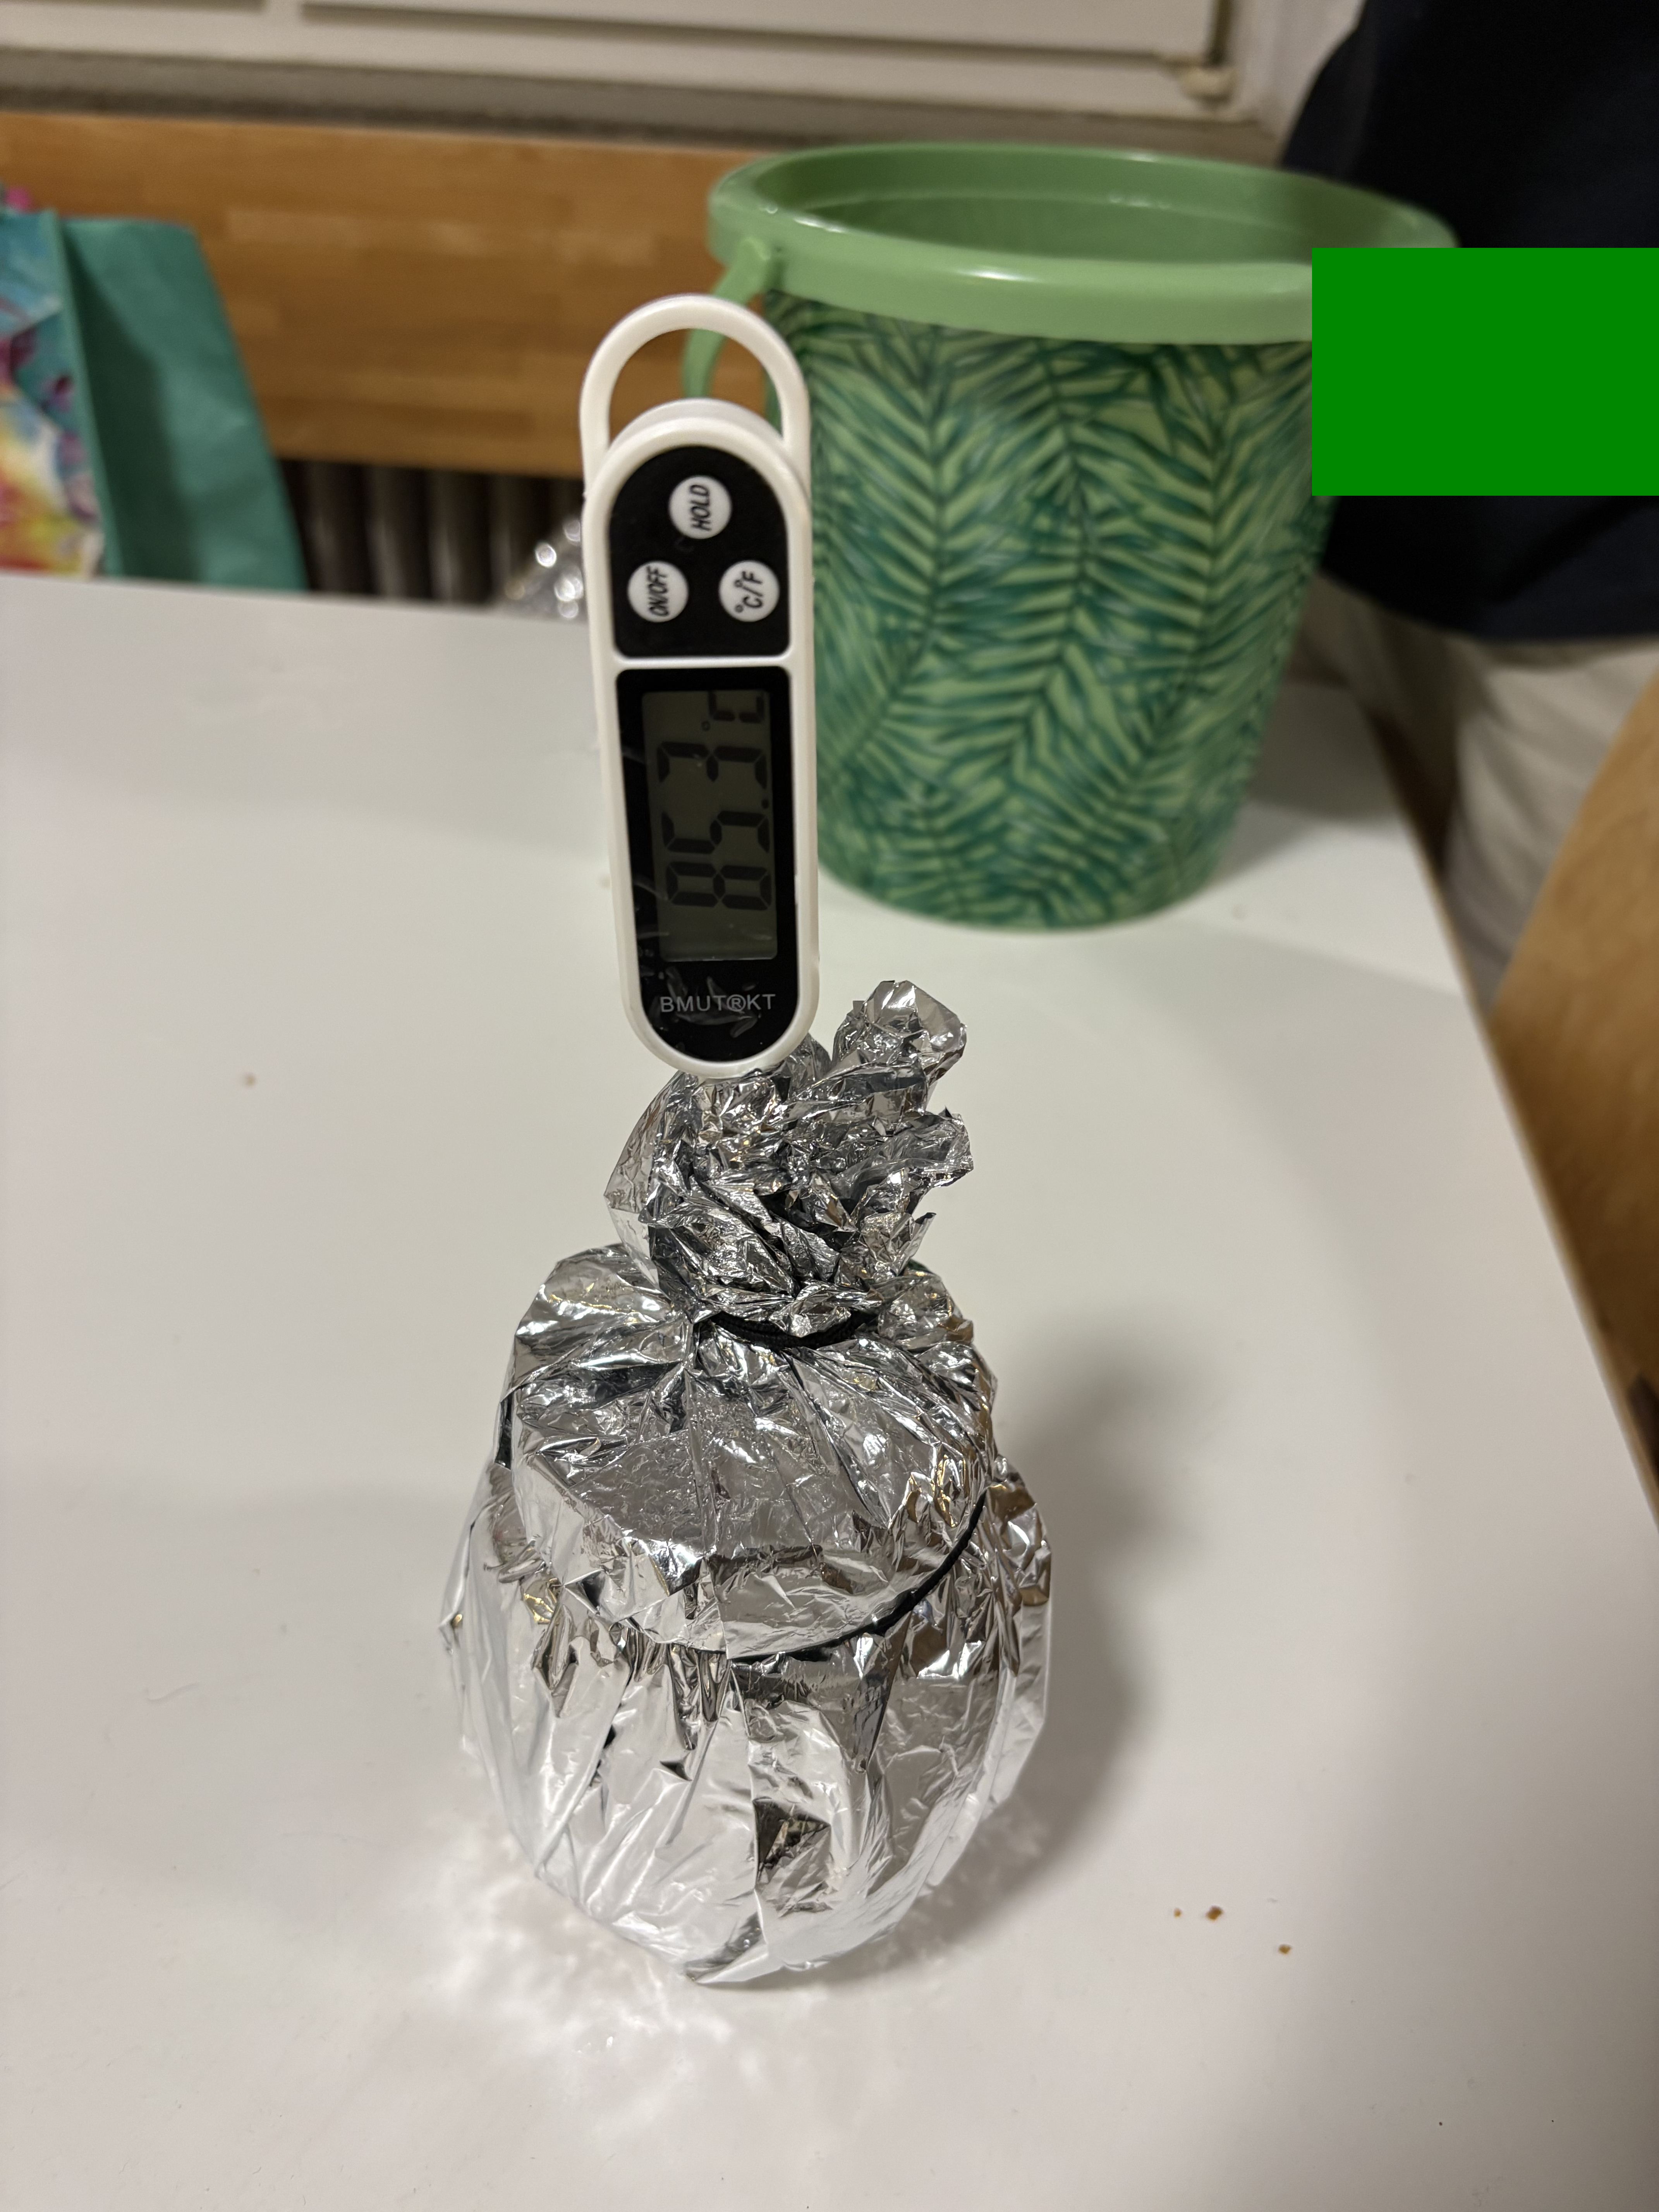
\includegraphics[height=42mm]{Onlymylar.jpg}\\[-1mm]\small C. Mylar
\end{minipage}\hfill
\begin{minipage}[t]{0.235\textwidth}\centering
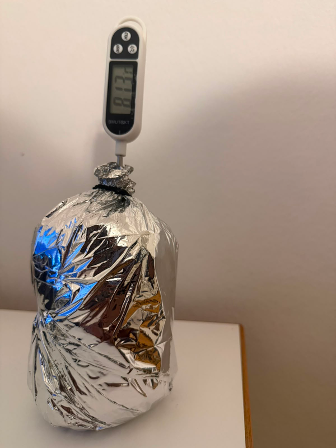
\includegraphics[height=42mm]{full-mli.png}\\[-1mm]\small D. Multilayer assembly
\end{minipage}
\caption{Standard four-configuration comparison assemblies.}
\end{figure}

\subsection{Multilayer assembly sequence}

\begin{enumerate}
  \item Wrap the dry glass jar uniformly with cotton. Avoid thick folds and leave the lid functional.
  \item Add bubble wrap with consistent overlap and intact air cells. Do not pull tape tight enough to crush the bubbles.
  \item Add Mylar as the outer layer with the shiny face outward. Close the top sufficiently to limit water circulation into the layers while leaving the display and lead junction dry.
  \item Confirm that the probe has not shifted and record the final layer order and approximate coverage.
\end{enumerate}

\begin{figure}[H]
\centering
\begin{minipage}{0.45\textwidth}\centering
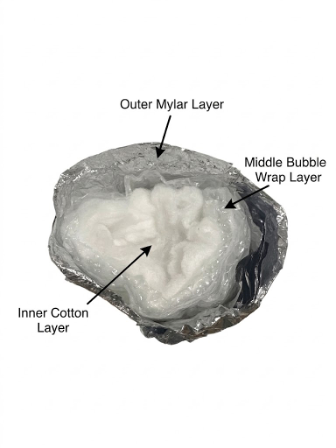
\includegraphics[height=54mm]{full-mli-parts.png}\\[-1mm]\small Layer order
\end{minipage}\hfill
\begin{minipage}{0.45\textwidth}\centering
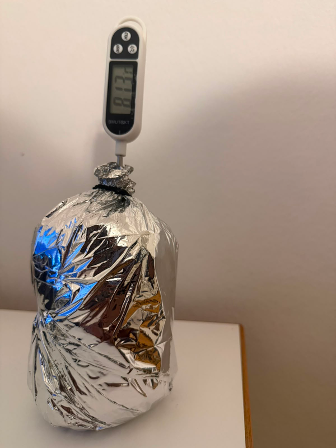
\includegraphics[height=54mm]{full-mli.png}\\[-1mm]\small Completed multilayer assembly
\end{minipage}
\caption{Educational multilayer test assembly. It is inspired by thermal-control principles but is not flight-qualified MLI.}
\end{figure}

\Needspace{8\baselineskip}
\section{Experimental procedure}

The preferred class arrangement is four teams running in parallel. If one jar is reused, return it and the bath to the same measured initial conditions before each run.

{\small
\renewcommand{\arraystretch}{1.08}
\begin{longtable}{C{9mm}p{0.31\textwidth}p{0.53\textwidth}}
\toprule
\textbf{Step} & \textbf{Action} & \textbf{Method and acceptance point} \\
\midrule
\endhead
1 & Configure Mission Control & Select Bare, Bubble Wrap, Mylar, or Multilayer. Enter the measured $T_0$ and measured $T_{\mathrm{env}}$; run the prediction before collecting data. \\
2 & Prepare the bath & Maintain a well-mixed ice-water slurry. Record $T_{\mathrm{env}}$ immediately before immersion and again at the end. \\
3 & Prepare the capsule & Instructor adds exactly 100 mL of water at no more than $80.0\,^{\circ}\mathrm{C}$. Fit and close the prepared probe lid using the approved method. \\
4 & Verify starting conditions & Confirm the internal reading is stable and within the instructor's agreed tolerance. Reposition the probe only before the run. \\
5 & Immerse and record $T_0$ & Using gloves or tongs, lower the capsule until the external bath level is above the internal water level. Start the timer at immersion and immediately record $t=0$. Do not submerge the display or lead junction. \\
6 & Log 15 minutes & Record the internal temperature at $t=1,2,\ldots,15$ minutes. Do not squeeze, move, unwrap, press down, or shade one sample differently. Document a late or missed timestamp rather than inventing a value. \\
7 & Monitor controls & Observe the seal, bath level, bath temperature, probe position, and layer wetting. Stop for leakage, glass damage, unstable supports, or electrical exposure. \\
8 & End the run & At 15 minutes, record the final capsule and bath temperatures. Remove the capsule with gloves or tongs and place it in secondary containment. \\
9 & Enter and check data & Confirm 16 observations from 0 through 15 minutes. Export or transcribe the Mission Control results and retain the paper task sheet. \\
10 & Cool and clean & Allow jars to cool before unwrapping. Empty them at a sink; dry probes, jars, insulation, and the work surface before storage. \\
\bottomrule
\end{longtable}
}

\begin{figure}[H]
\centering
\begin{minipage}{0.47\textwidth}\centering
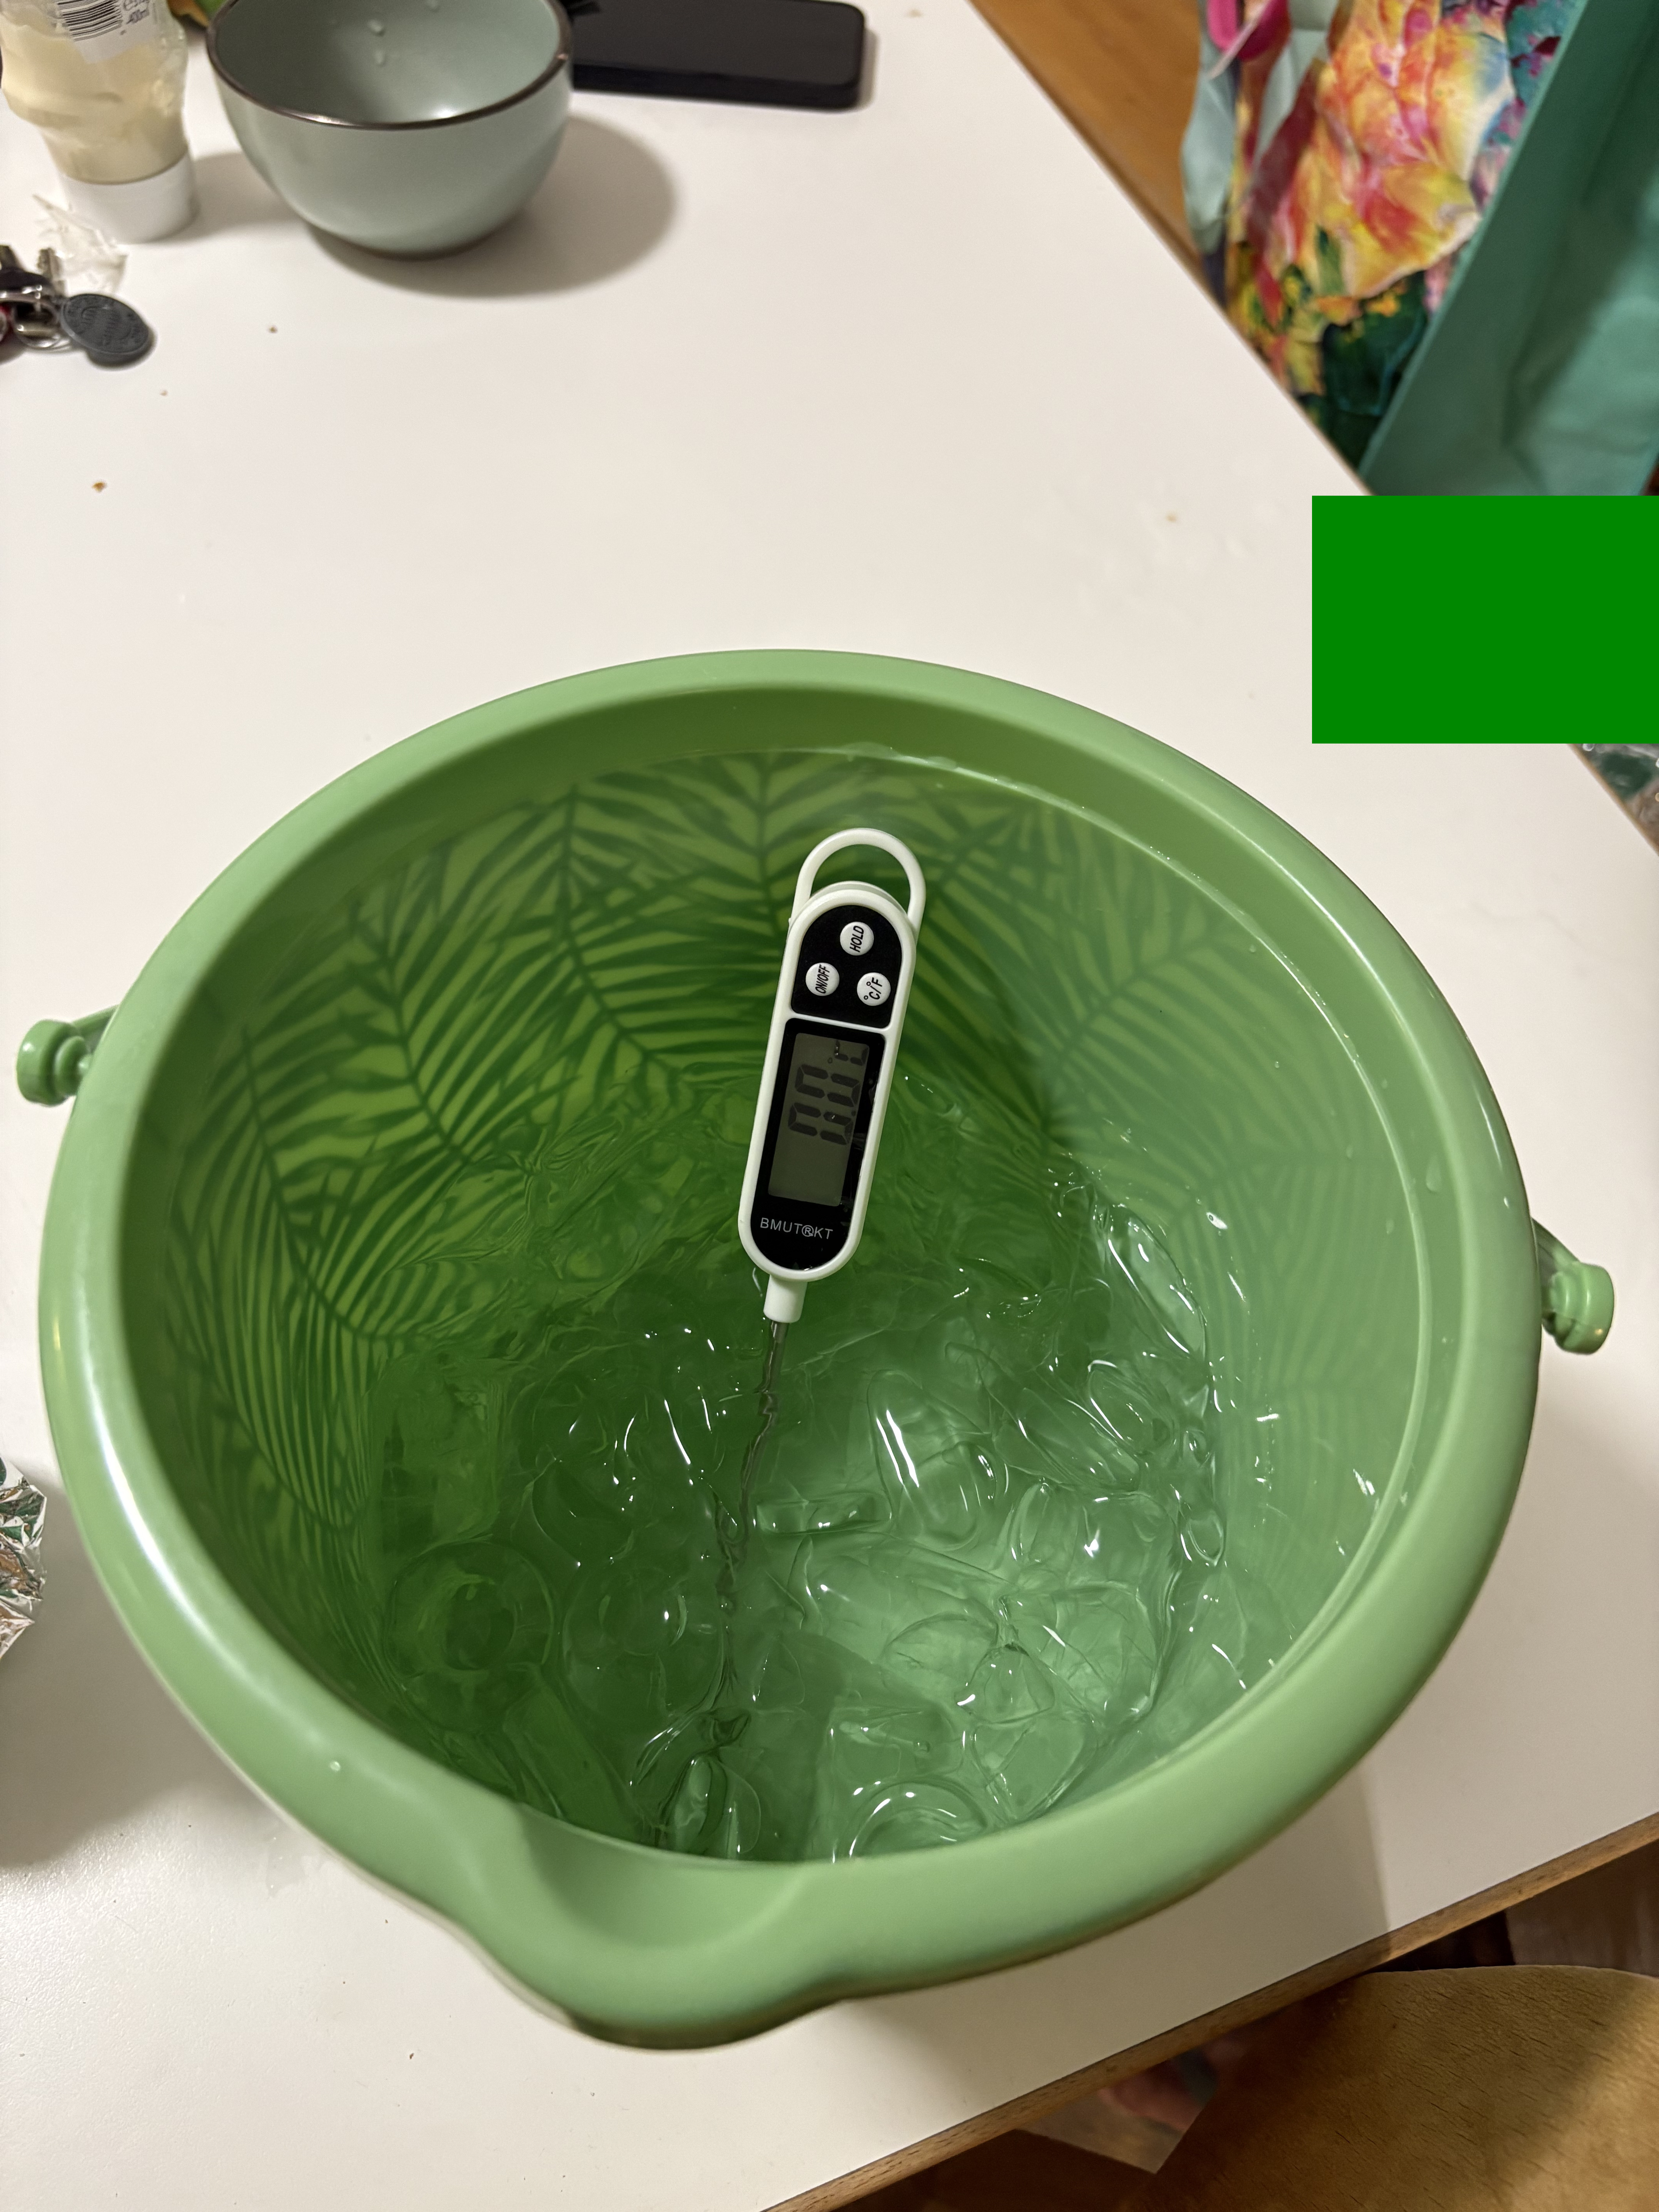
\includegraphics[height=63mm]{bathwater-0temp.jpg}\\[-1mm]\small Measure the actual bath boundary
\end{minipage}\hfill
\begin{minipage}{0.47\textwidth}\centering
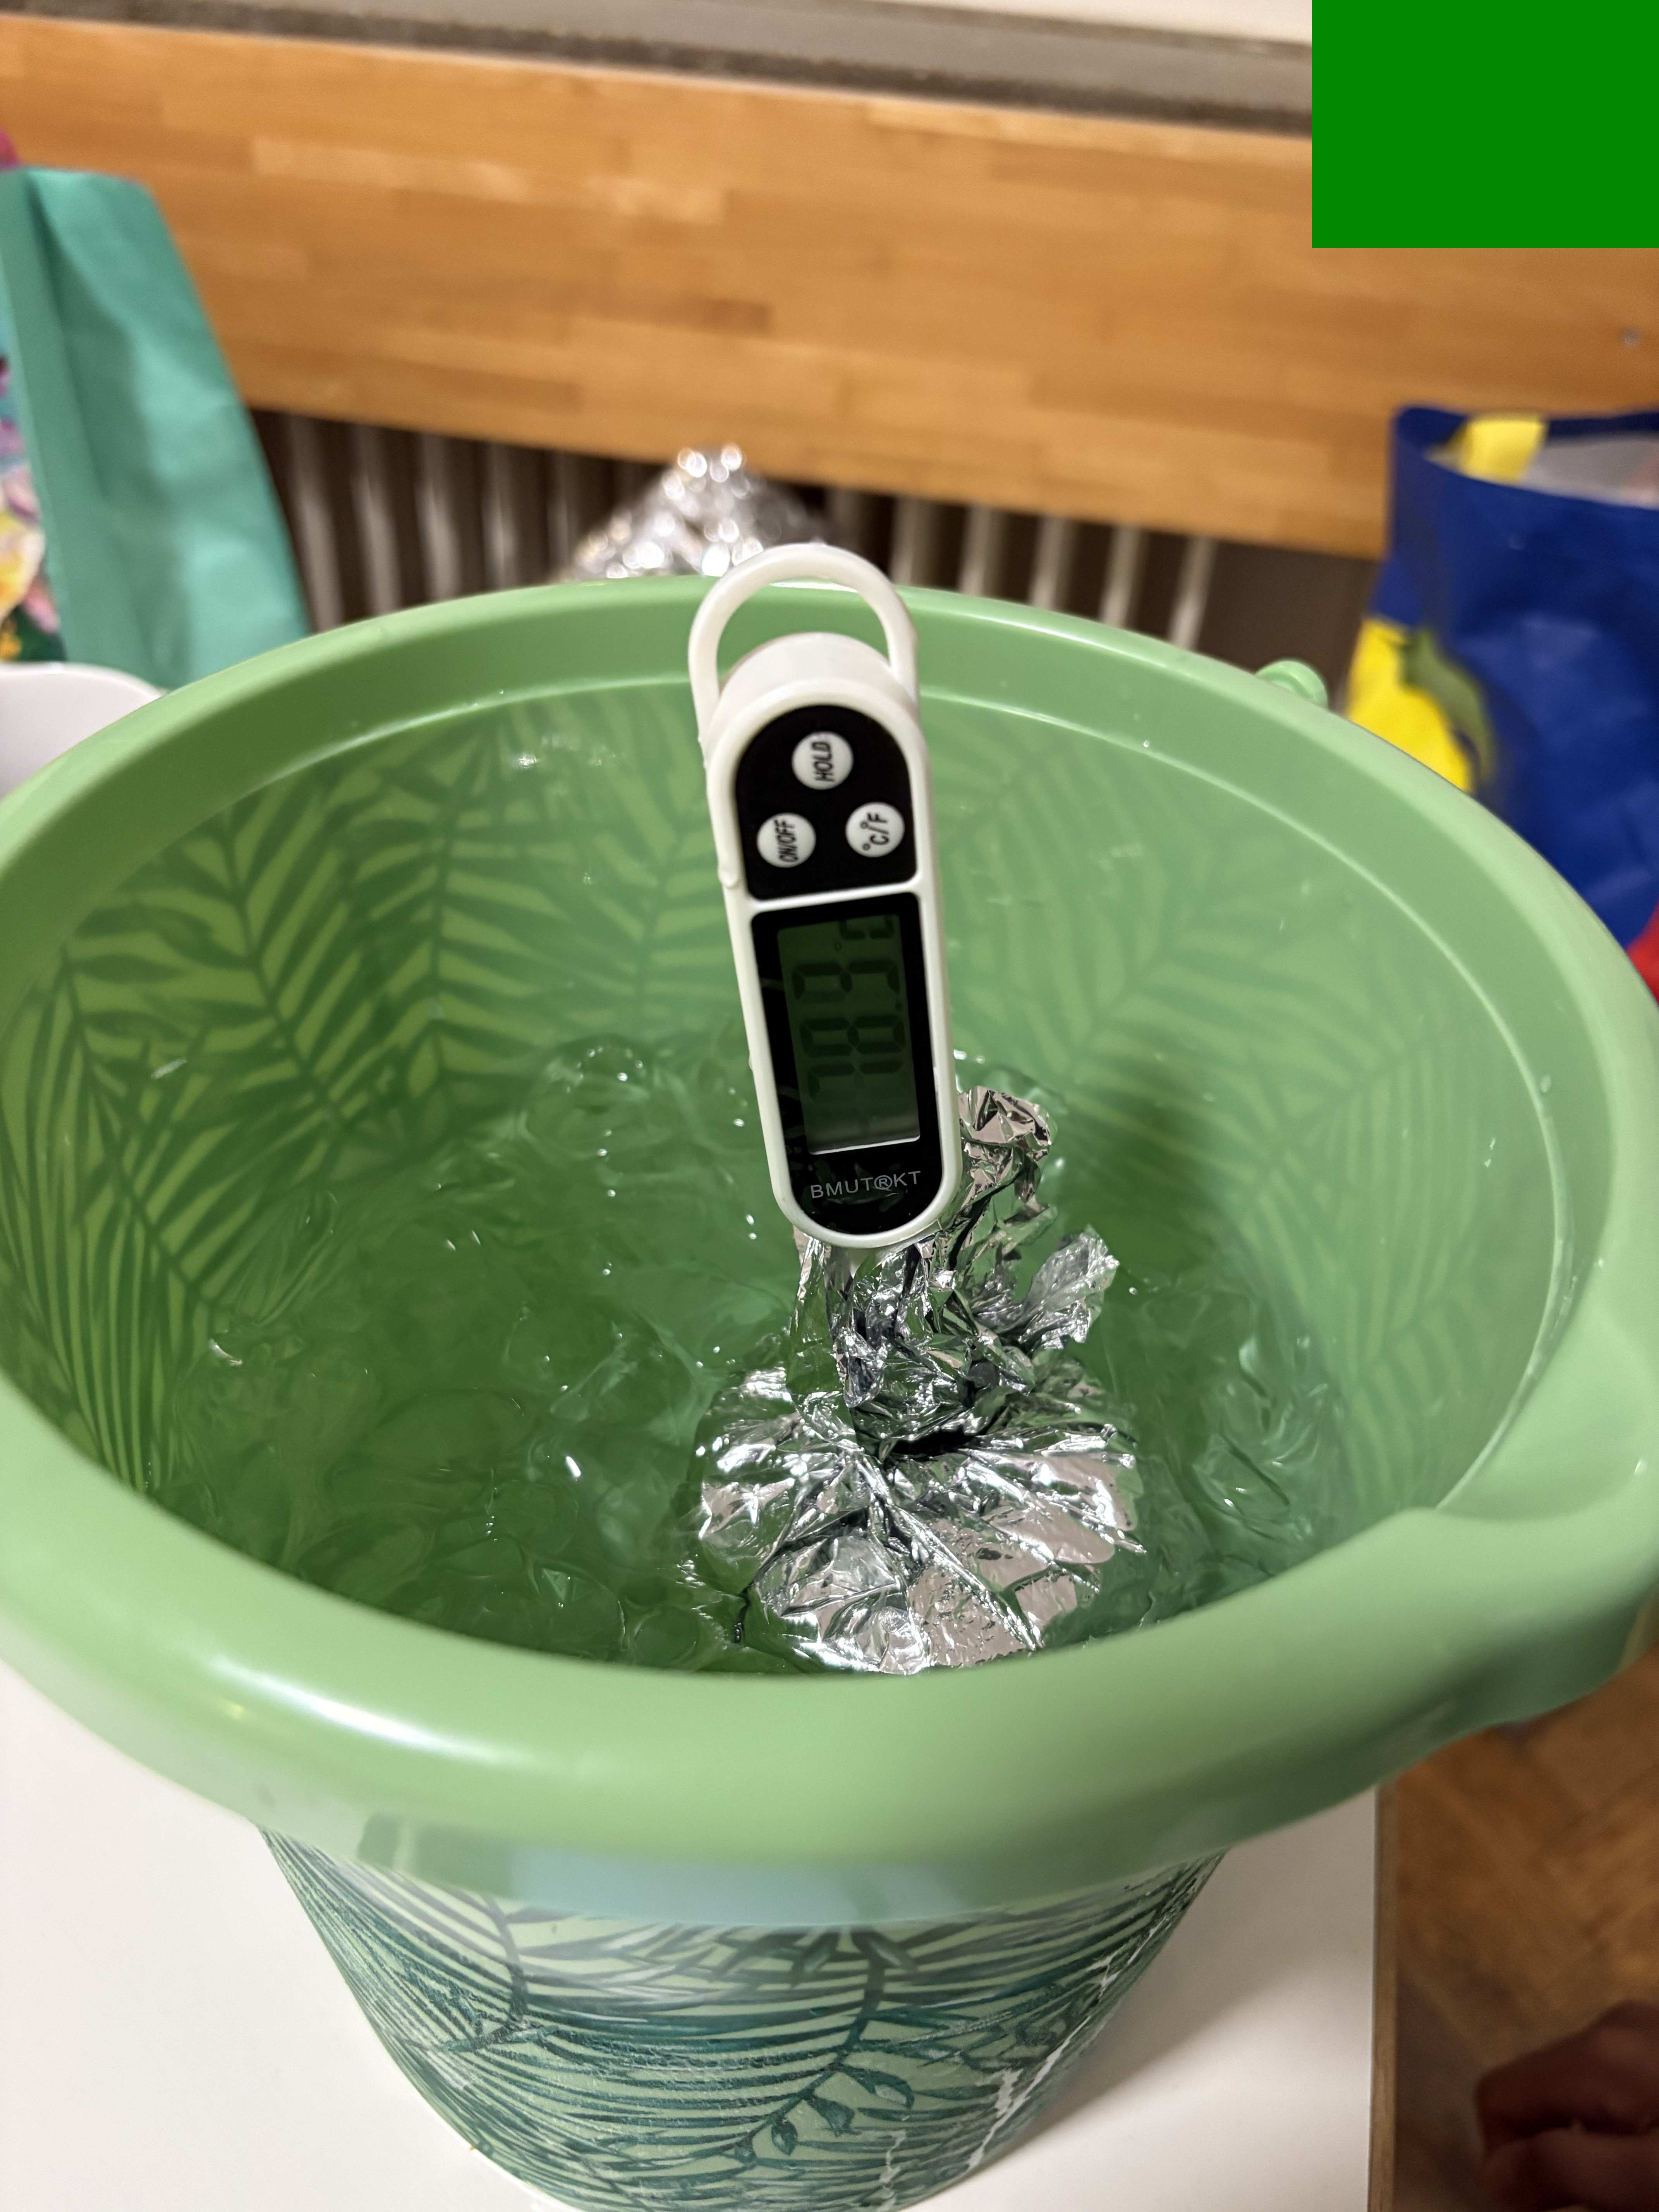
\includegraphics[height=63mm]{capsuleinside.jpg}\\[-1mm]\small Immerse to the internal water line
\end{minipage}
\caption{Cold-boundary verification and capsule immersion.}
\end{figure}

\begin{figure}[H]
\centering
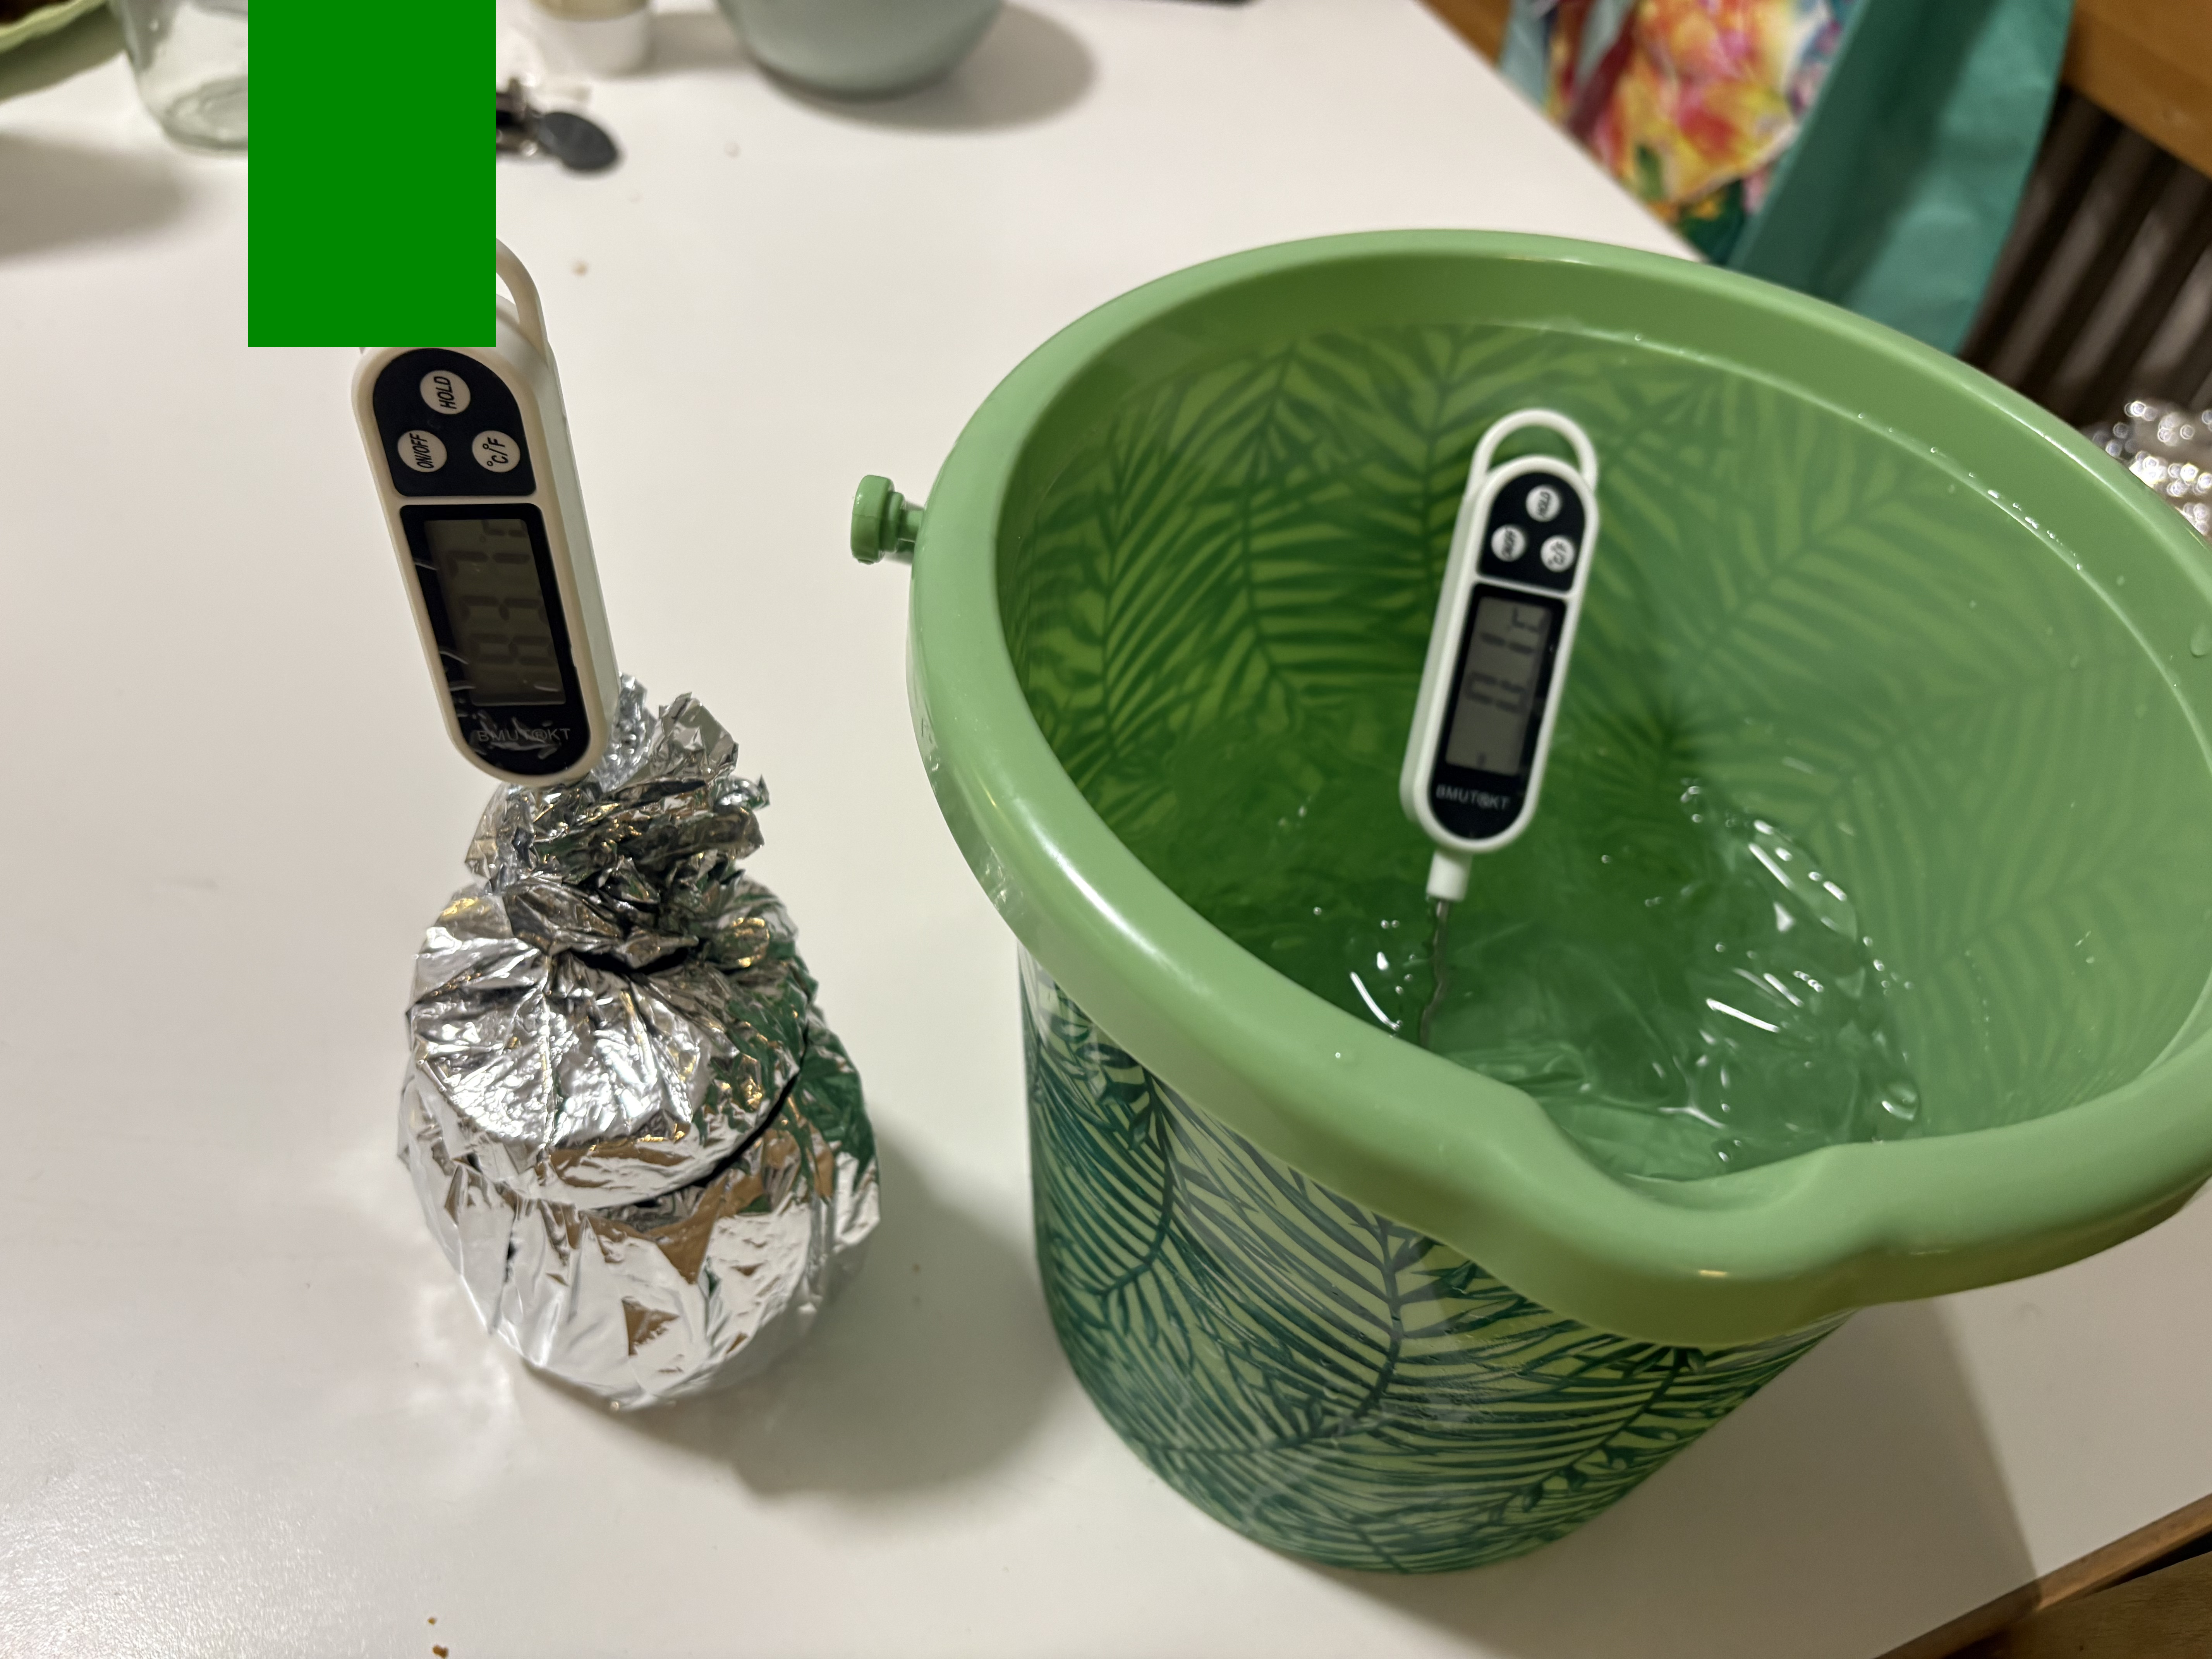
\includegraphics[width=0.90\textwidth]{setup.jpg}
\caption{Dry data station separated from the ice-water bath. Keep the thermometer display and electronics out of the water.}
\end{figure}

\Needspace{16\baselineskip}
\section{Data reduction and model comparison}

For observation $i$ at time $t_i$, use the actual measured bath temperature as $T_{\mathrm{env}}$:

\begin{align}
T_{\mathrm{model}}(t) &= T_{\mathrm{env}} + (T_0-T_{\mathrm{env}})e^{-kt},\\
r_i &= T_{\mathrm{obs},i}-T_{\mathrm{model},i},\\
\mathrm{MAE} &= \frac{1}{n}\sum_{i=1}^{n}|r_i|,\\
k_{\mathrm{est}} &= -\frac{1}{t}\ln\!\left(\frac{T(t)-T_{\mathrm{env}}}{T_0-T_{\mathrm{env}}}\right).
\end{align}

Use $n=16$ when all readings from $t=0$ through $15$ minutes are included. State a different $n$ explicitly if a reading is invalid or missing. Report $k$ in min$^{-1}$ and MAE in $^{\circ}\mathrm{C}$. Compare MAE with instrument accuracy and between-run variation; do not convert MAE into an invented percentage score.

\begin{figure}[H]
\centering
\begin{minipage}{0.49\textwidth}\centering
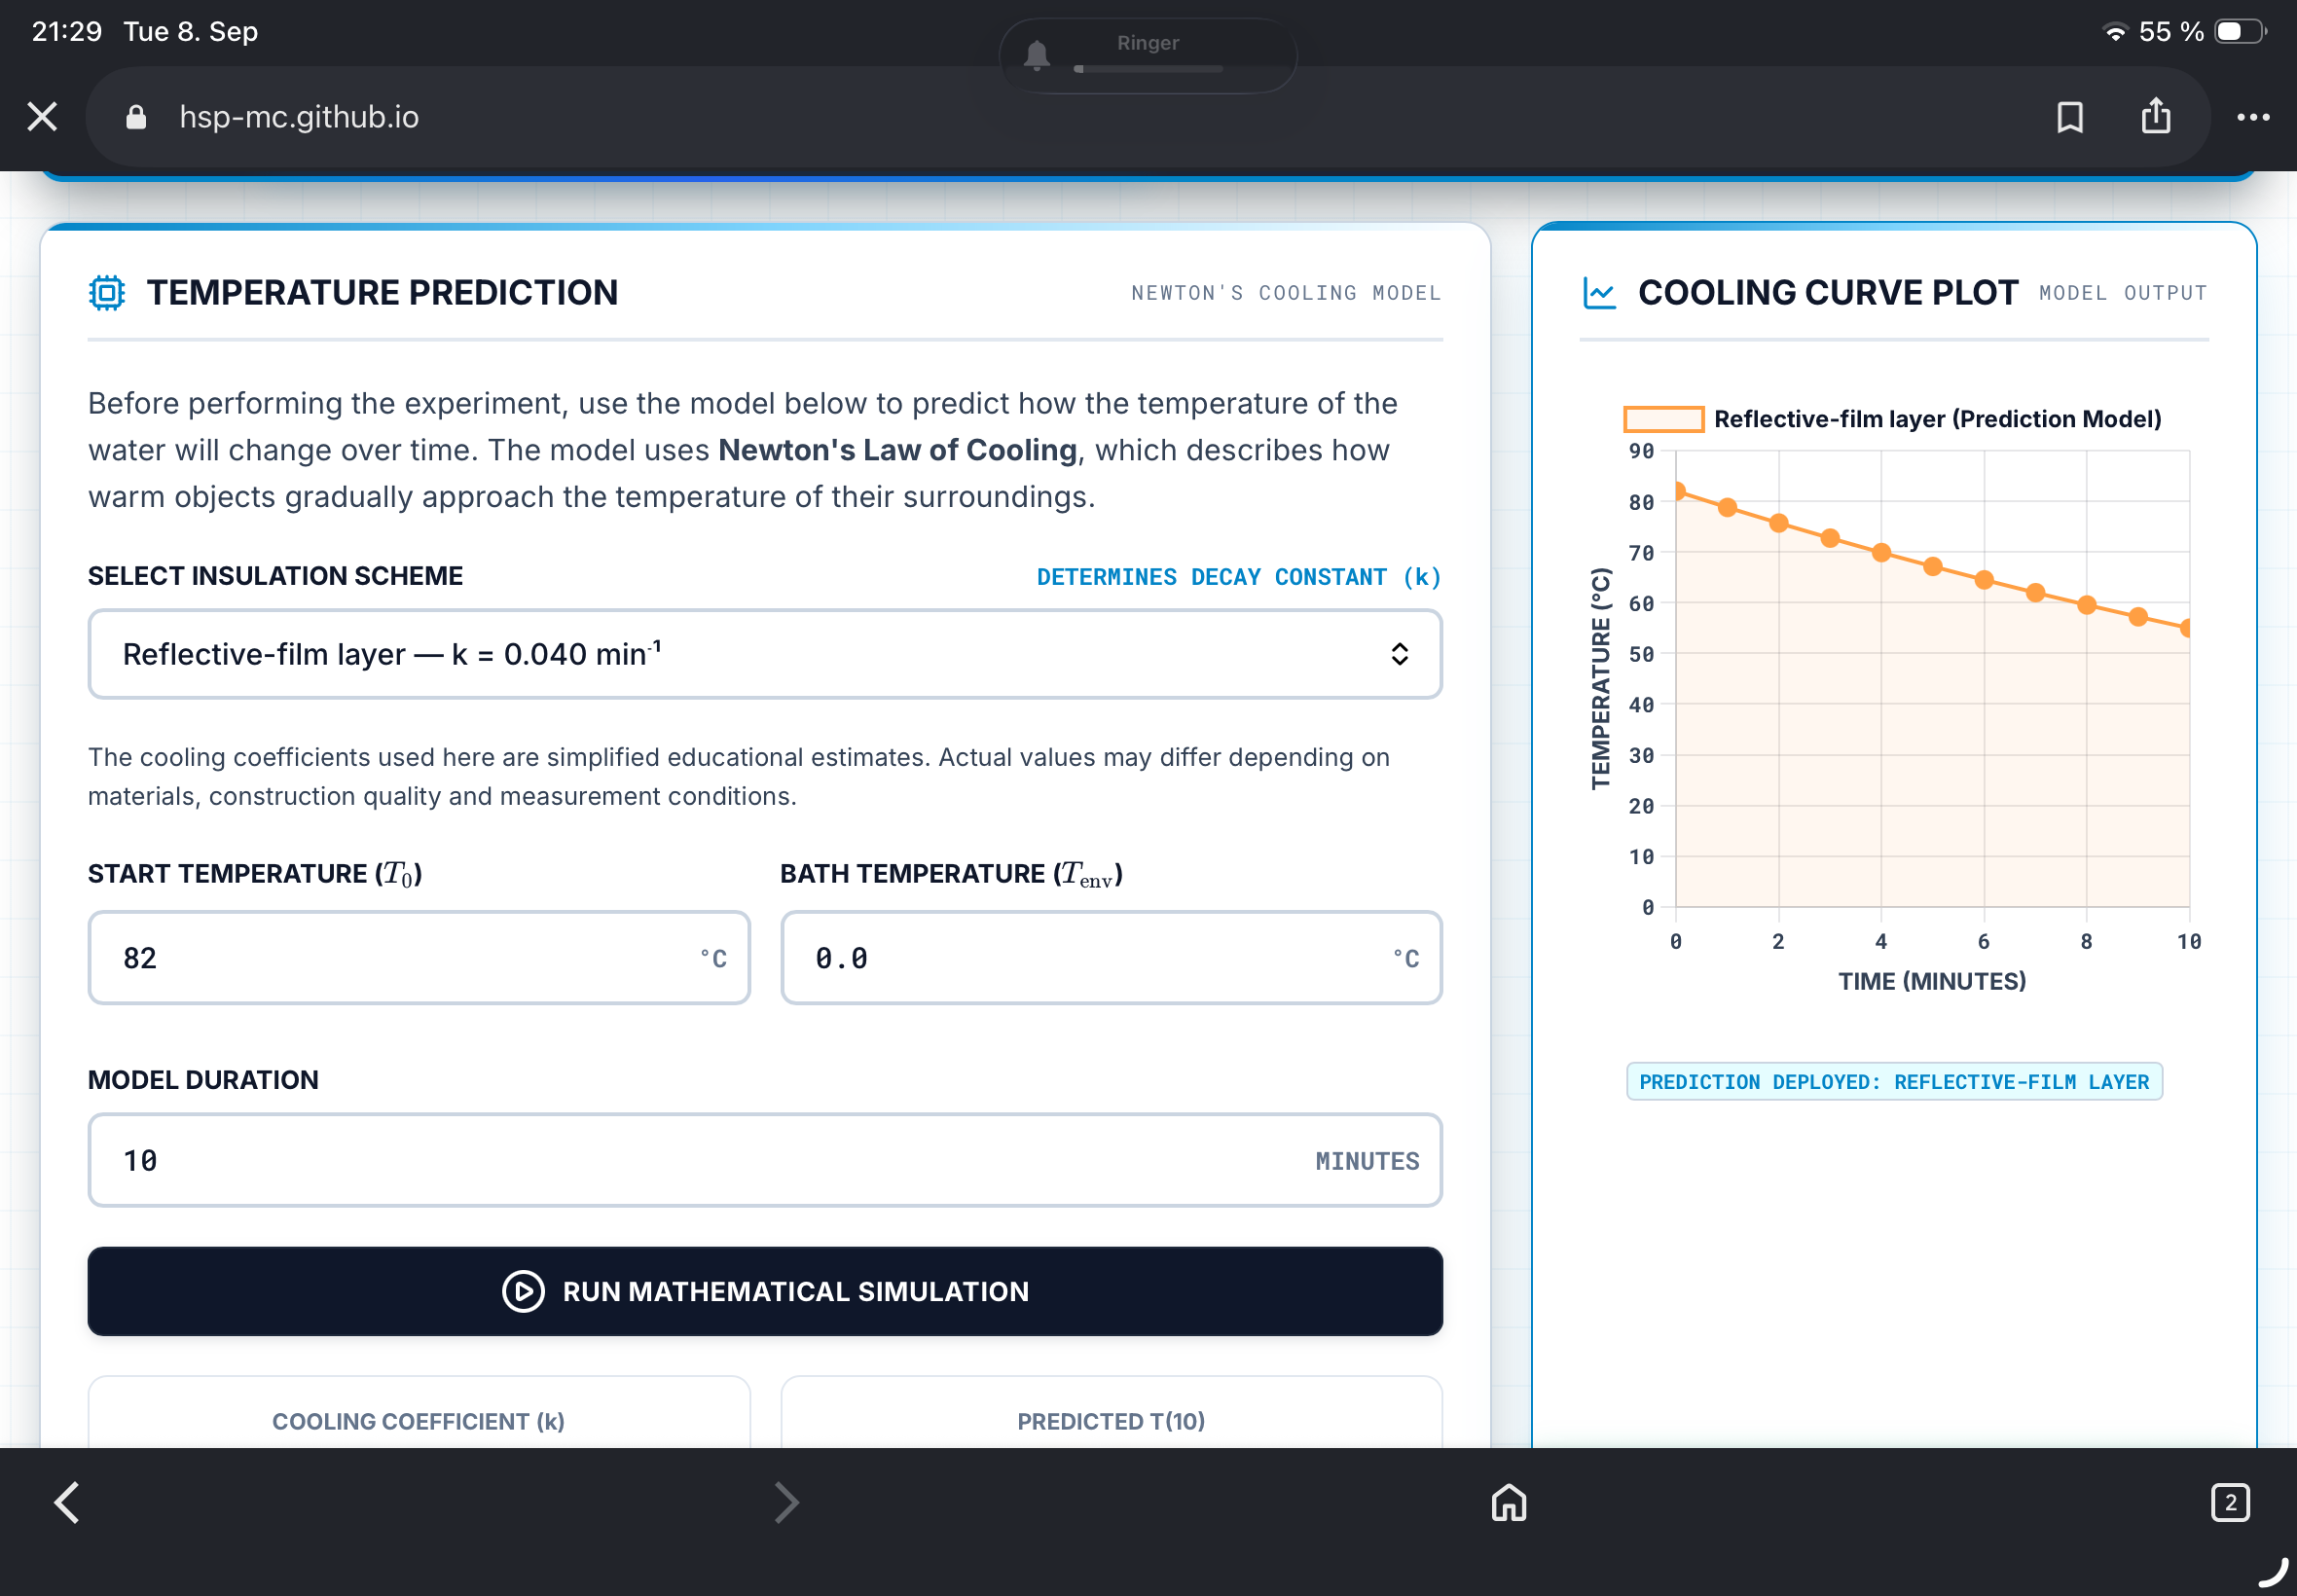
\includegraphics[width=\linewidth]{website-setting up.PNG}\\[-1mm]\small Configure the current Mission Control model
\end{minipage}\hfill
\begin{minipage}{0.49\textwidth}\centering
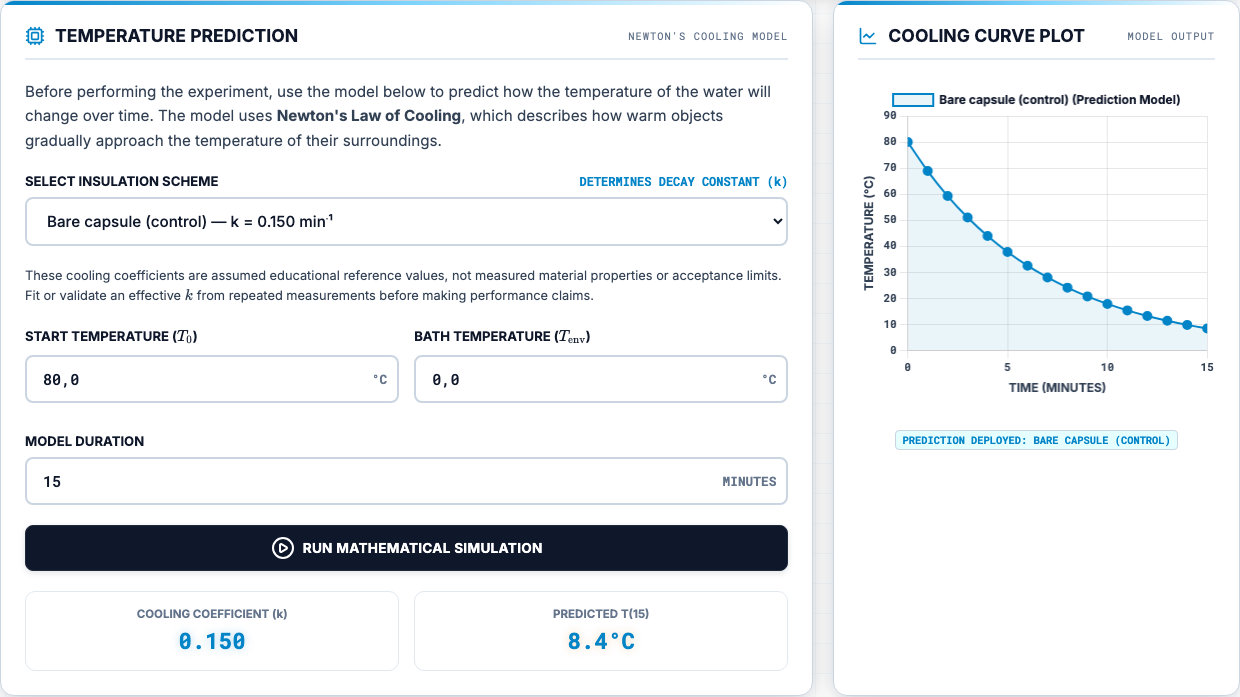
\includegraphics[width=\linewidth]{predicted-curve.png}\\[-1mm]\small Preserve the prediction before measurement
\end{minipage}
\caption{Mission Control setup and reference prediction.}
\end{figure}

\begin{figure}[H]
\centering
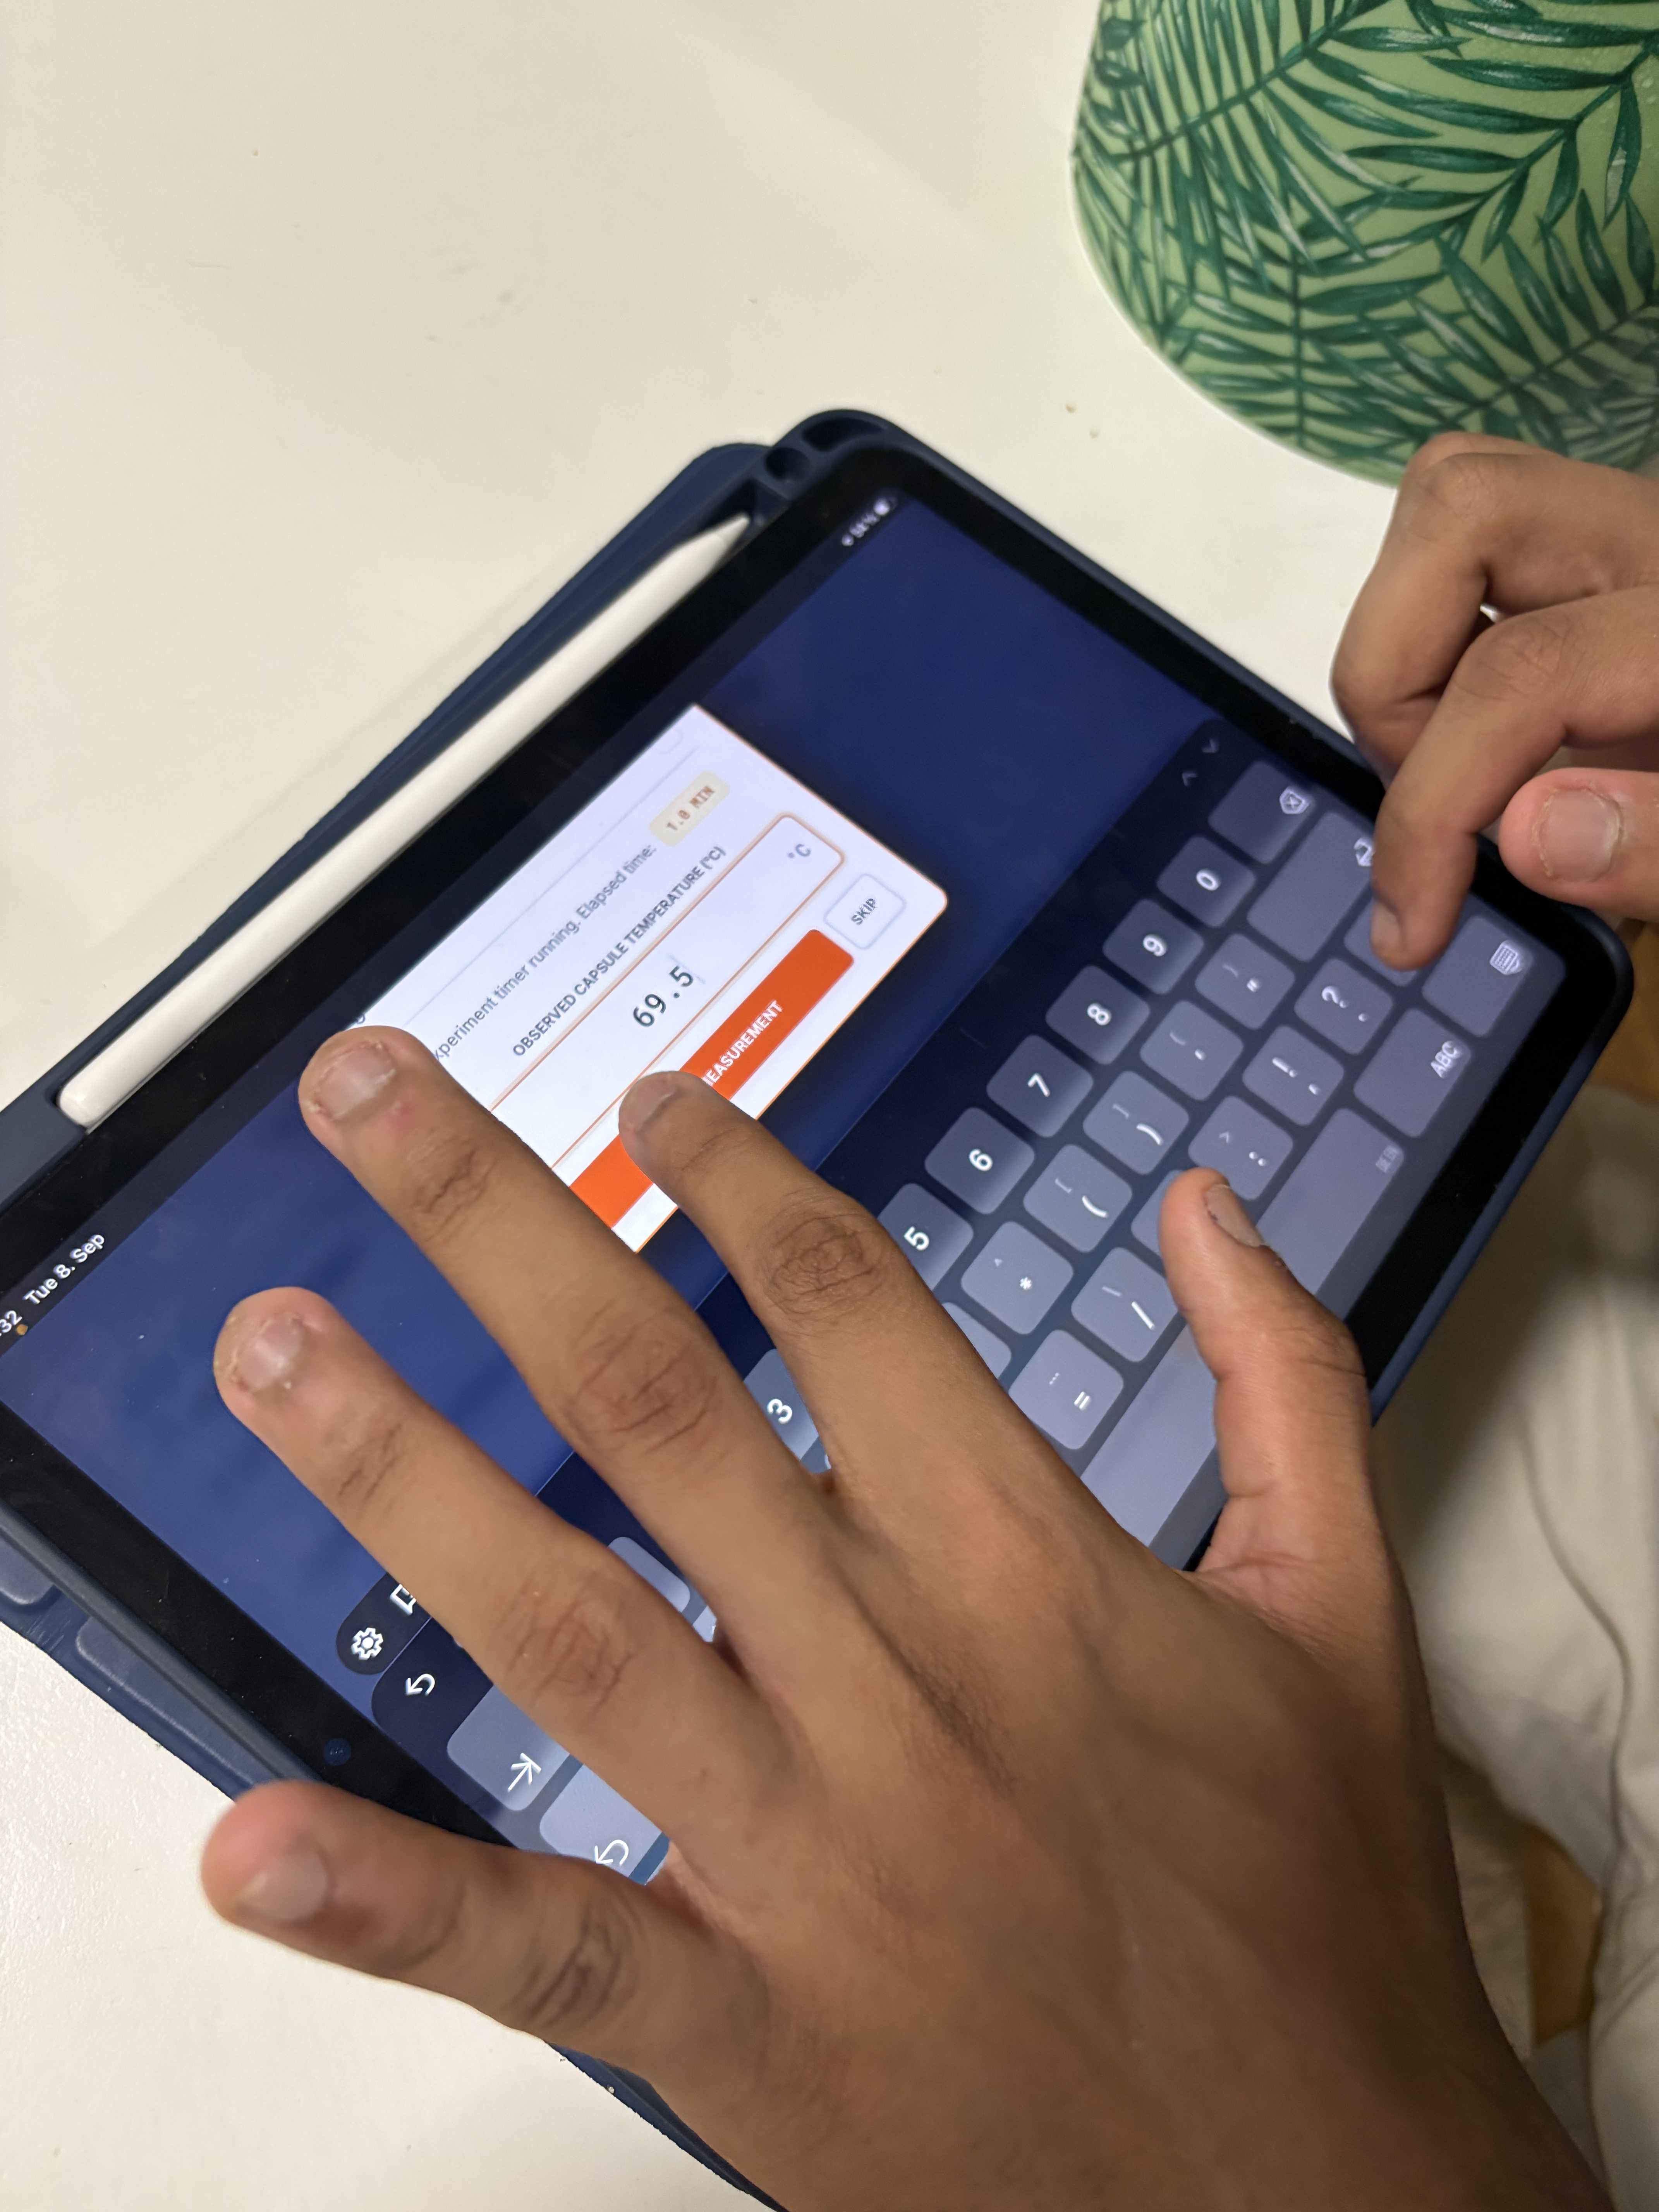
\includegraphics[height=0.28\textheight]{input temp.jpg}
\caption{Manual temperature entry. Record the observation at the actual timestamp and retain the raw log.}
\end{figure}

\Needspace{8\baselineskip}
\section{Quality controls and troubleshooting}

\begin{tabularx}{\textwidth}{p{0.26\textwidth}Yp{0.29\textwidth}}
\toprule
\textbf{Observation} & \textbf{Likely cause} & \textbf{Response} \\
\midrule
Sudden temperature fall & Cold-water leakage; probe touching the glass; sample moved; severe internal mixing. & Stop if leakage is suspected. Mark the point invalid, inspect the jar and seal after cooling, and repeat safely. \\
Starting temperatures differ & Filling or transfer delay; inconsistent water source; different preconditioning. & Do not rank by final temperature alone. Repeat within tolerance or compare fitted $k$ and normalized temperature excess. \\
Bath warms during the run & Too little ice, poor mixing, or high room temperature. & Measure the actual bath temperature and update $T_{\mathrm{env}}$; document drift as uncertainty. \\
Mylar performs poorly & Direct liquid contact, tears, water entry, or no insulating spacer. & Treat the result as system behavior under immersion, not proof that reflective insulation is universally ineffective. \\
MLI result varies between teams & Different cotton thickness, crushed bubbles, open top, or inconsistent overlap. & Photograph and record layer construction; rebuild to the standard sequence before comparing. \\
High MAE & Wrong model selection, wrong $T_0$ or $T_{\mathrm{env}}$, irregular timing, probe shift, leakage, or reference $k$ not calibrated to the hardware. & Check inputs and raw timestamps first; then discuss model limitations and repeatability. \\
\bottomrule
\end{tabularx}

\Needspace{8\baselineskip}
\section{Acceptance checklist}

\begin{tabularx}{\textwidth}{C{12mm}Y}
\toprule
\textbf{Done} & \textbf{Completion criterion} \\
\midrule
$\square$ & Four undamaged 100 mL glass jars with prepared probe lids were used. \\
$\square$ & Every lid passed a cold-water leak test before hot filling. \\
$\square$ & Initial water temperature did not exceed $80.0\,^{\circ}\mathrm{C}$ and the actual $T_0$ was recorded. \\
$\square$ & The actual ice-bath temperature was measured and entered as $T_{\mathrm{env}}$. \\
$\square$ & Probe depth, water volume, immersion depth, timing, and layer coverage were controlled. \\
$\square$ & Every valid trial contains 16 time-temperature pairs from 0 through 15 minutes. \\
$\square$ & Graphs show units, labels, legend, observed data, and model data on the same time axis. \\
$\square$ & Residuals and MAE were calculated with the stated number of valid observations. \\
$\square$ & Conclusions distinguish measured system behavior, build quality, uncertainty, and model assumptions. \\
$\square$ & All jars, probes, insulation, baths, and work surfaces were cooled, emptied, dried, and stored safely. \\
\bottomrule
\end{tabularx}

\Needspace{12\baselineskip}
\section{Document synchronization record}

This document uses the same experiment definition as the current project materials: 100 mL glass jars with prepared probe lids; a measured ice-water boundary; four standard configurations; a 15-minute run with observations at $t=0$ through $15$ minutes; Newtonian cooling; residuals and MAE; and the reference constants in Mission Control.

\begin{tabularx}{\textwidth}{p{0.37\textwidth}Y}
\toprule
\textbf{Aligned source} & \textbf{Controlled content} \\
\midrule
SPHERE Mission Control Student Manual & Hardware, four configurations, layer sequence, experiment stages, model equations, and MAE. \\
SPHERE Mission Control Teacher Manual & Safety limits, risk controls, 60-minute lesson flow, model constants, and instructor acceptance criteria. \\
Student Task Sheet & Sixteen-point log, graph, residual and MAE fields, and ten inquiry prompts. \\
SPHERE Mission Control Flashcards & Terminology for heat transfer, effective cooling constant, boundary condition, and multilayer mechanism. \\
Mission Control web application & Configuration names, model constants, 15-minute timer, manual telemetry entry, and MAE output. \\
\bottomrule
\end{tabularx}

\note{If any current project interface or manual is revised, update this SOP's configuration names, equations, safety controls, and acceptance checklist in the same release.}

\small\textbf{Limit of use.} This activity demonstrates comparative thermal behavior under classroom conditions. It does not certify any material or assembly for aerospace, pressure-vessel, fire-protection, or personal-protective use.

\end{document}
